% Copyright (C) 2017 by SIB Swiss Institute of Bioinformatics, Julien Dorier and Dimos Goundaroulis.
% 
% This file is part of project Knoto-ID.
% 
% Knoto-ID is free software: you can redistribute it and/or modify
% it under the terms of the GNU General Public License as published by
% the Free Software Foundation, either version 2 of the License, or
% (at your option) any later version.
% 
% Knoto-ID is distributed in the hope that it will be useful,
% but WITHOUT ANY WARRANTY; without even the implied warranty of
% MERCHANTABILITY or FITNESS FOR A PARTICULAR PURPOSE.  See the
% GNU General Public License for more details.
% 
% You should have received a copy of the GNU General Public License
% along with Knoto-ID.  If not, see <http://www.gnu.org/licenses/>.

\documentclass[a4paper,10pt]{article}

\usepackage[margin=2cm]{geometry}

\usepackage{xcolor}
\definecolor{lightgrey}{rgb}{0.9,0.9,0.9}
\definecolor{lightergrey}{rgb}{0.97,0.97,0.97}


\usepackage[T1]{fontenc}
\usepackage[utf8]{inputenc}
\usepackage{graphicx}
\usepackage{bm}

%%fonts
\usepackage{lmodern} %font type I (vectoriel)

\renewcommand*{\familydefault}{\sfdefault} 

\usepackage[nosort]{cite}
\usepackage[colorlinks=true,urlcolor=blue,linkcolor=black]{hyperref} 


\input{variables_cmake.tex}
\graphicspath{\cmakefigurepath}


\renewcommand{\labelitemii}{$\circ$}

\usepackage[bf]{caption}
\setlength{\captionmargin}{10mm}




\usepackage[protrusion=false]{microtype} %protrusion=false, to avoid problem of alignment in ttfamily when line start with "-"
\DisableLigatures{family=tt*} %%to avoid -- replaced by en-dash in ttfamily

\usepackage{verbatim}
\usepackage{adjustbox}
\newenvironment{lstlisting}%
               {\par\noindent\adjustbox{margin=1ex,bgcolor=lightgrey,margin=0ex \medskipamount}\bgroup\minipage\linewidth\small\ttfamily\verbatim}%
               {\endverbatim\endminipage\egroup\\}
               
\newenvironment{lstlistingsmall}%
               {\par\noindent\adjustbox{margin=1ex,bgcolor=lightgrey,margin=0ex \medskipamount}\bgroup\minipage\linewidth\footnotesize\ttfamily\verbatim}%
   {\endverbatim\endminipage\egroup\\}
   
\newenvironment{lstlistingverysmall}%
               {\par\noindent\adjustbox{margin=1ex,bgcolor=lightgrey,margin=0ex \medskipamount}\bgroup\minipage\linewidth\scriptsize\ttfamily\verbatim}%
               {\endverbatim\endminipage\egroup\\}
                  
                  
\newcommand{\lstinline}[1]{{\colorbox{lightergrey}{\ttfamily\detokenize{#1}}}} %with colorbox => does not break lines
\newcommand{\lstinlineT}[1]{{\colorbox{lightergrey}{\ttfamily #1}}} %with colorbox => does not break lines

\usepackage{tikz}
\usepackage{subfig}
\usepackage{amsfonts}
\usepackage{mathtools}

\setlength{\parindent}{0mm} 
\setcounter{secnumdepth}{3}
\setcounter{tocdepth}{4}



%%%%%%%%%%%%%%%%%%%%%%%%%%%%%%%%%%%%%%%%%%%%%%%%%%%%%%%
%%%%%%%%%%%%%%%%%%%%%%%%%%%%%%%%%%%%%%%%%%%%%%%%%%%%%%%
%%%%%%%%%%%%%%%%%%%%%%%%%%%%%%%%%%%%%%%%%%%%%%%%%%%%%%%

\begin{document}

%%%%%% title %%%%%%%%%
\begin{titlepage}
  \begin{center}
\vspace*{30mm}
 {\Huge \bf Knoto-ID}\\
\vspace*{5mm}
\LARGE{Topological invariants of open curves\\
  using the concept of knotoids}\\
\vspace*{20mm}
\LARGE{\bf User guide}\\
\vspace*{5mm}
\normalsize Version \cmakeversion \ (\today)\\
\vspace*{10mm}
Julien Dorier$^{1,3}$, Dimos Goundaroulis$^{2,3}$\\
\vspace*{5mm}
\small
$^1$ Vital-IT, SIB Swiss Institute of Bioinformatics, Switzerland.\\
$^2$ SIB Swiss Institute of Bioinformatics, Switzerland.\\
$^3$ Center for Integrative Genomics, University of Lausanne, Switzerland.\\
\end{center}
\end{titlepage}
\newpage

\tableofcontents
\newpage


\section{Introduction}
The backbone of most proteins forms an open curve.  To study their
entanglement, a common strategy consists in searching for the presence
of knots in their backbones using topological invariants.  However,
this approach requires to close the curve into a loop, which alters
its geometry.  {\it Knoto-ID} allows evaluating the
entanglement of open curves without the need to close them, using the
recent concept of knotoids\cite{turaev,guka} which is a generalization
of classical knot theory to open curves.  {\it Knoto-ID} can analyse
the global topology of the full chain as well as the local topology by
exhaustively studying all subchains or only determining the knotted
core.  The use of {\it Knoto-ID} is not limited to proteins, it can be
used to analyse any open curve in 3D space such as chromosomes,
synthetic polymers, random walks, etc.

{\it Knoto-ID} is a collection of command line tools with three executables (\lstinline{polynomial_invariant}, \lstinline{knotted_core} and  \lstinline{convert_diagram}) and five helper scripts (\lstinline{pdb_to_xyz.R}, \lstinline{plot_3D_curve.R}, \lstinline{plot_projection_map.R}, \lstinline{plot_knotted_core.R} and \lstinline{plot_diagram.R}):
\begin{itemize}
\item \lstinline{polynomial_invariant} computes the following polynomial invariants: the classical Jones polynomial for knots (closed curves), the Jones polynomial for knotoids (open curves projected on a sphere), the Turaev loop bracket for knotoids (open curves projected on a plane), the arrow polynomial (open curves projected on a sphere) and the loop arrow polynomial (open curves projected on a plane). \lstinline{polynomial_invariant} can output lists of polynomials obtained with multiple projection directions, which can be used to generate projection maps similar to those presented in\cite{gound}. A simple helper script \lstinline{plot_projection_map.R} is included with {\it Knoto-ID} to create such projection maps using the output of \lstinline{polynomial_invariant}.
\item \lstinline{knotted_core} computes the knotted core of an open or closed curve. It can also be used to evaluate the dominant invariant polynomials for all subchains of the input curve. This data can be used to generate fingerprint matrices\cite{yeates, sulkowska2012, gound} (for open curves) or disk matrices\cite{rawdon} (for closed curves). A simple script \lstinline{plot_knotted_core.R} is included with {\it Knoto-ID} to create such fingerprint or disk matrices using the output produced by \lstinline{knotted_core}.
\item \lstinline{convert_diagram} convert diagrams from/to PD codes, extended Gauss codes and piecewise linear curve (xyz). In particular, the xyz output format can be used to draw the diagram with the helper script \lstinline{plot_diagram.R} which is included with {\it Knoto-ID}.
\item \lstinline{pdb_to_xyz.R} is a simple helper script to convert the backbone of proteins given in pdb format\cite{pdb} to piecewise linear curves in xyz format that can be used as input by {\it Knoto-ID}.
\item \lstinline{plot_3D_curve.R} is a simple helper script to convert piecewise linear curves from xyz format to webGL format\cite{webgl} that can then be viewed interactively in compatible web browsers.
\end{itemize}
This document starts with a tutorial (section ``\ref{sec:tutorial} \nameref{sec:tutorial}'') where examples of use cases are shown. More details on the executables and their arguments, as well as a description of the file formats are given in section ``\ref{sec:reference} \nameref{sec:reference}''.  Mathematical concepts, definitions and choices of conventions are given in section ``\ref{sec:theory} \nameref{sec:theory}''.

\subsection{Credit}
If you use this software for a publication, please cite:\\
J. Dorier, D. Goundaroulis, F. Benedetti and A. Stasiak, "Knoto-ID: a tool to study the entanglement of open protein chains using the concept of knotoids", Bioinformatics 34(19):3402--3404, 2018.

If you use the knotoid classification\footnote{using internal database with \lstinline{--names-db=internal} or files \lstinline{examples/knotoid_names_planar.txt}, \lstinline{examples/knotoid_names_sphere.txt}, \lstinline{examples/knotoid_names_planar_arrow.txt} or \lstinline{examples/knotoid_names_sphere_arrow.txt}}, please cite:\\
D. Goundaroulis, J. Dorier and A. Stasiak, "A systematic classification of knotoids on the plane and on the sphere", arXiv:1902.07277 [math.GT].

\subsection{Installation}
The latest precompiled binary distribution is available for Linux, Mac OS X and Windows at
\url{https://github.com/sib-swiss/Knoto-ID/releases/latest}

Decompress Knoto-ID:
\begin{lstlisting}
$ tar -xf Knoto-ID-<version>.tar.gz 
\end{lstlisting}
Go in the Knoto-ID directory
\begin{lstlisting}
$ cd Knoto-ID-<version>/ 
\end{lstlisting}

{\it Knoto-ID} is organized into four directories:
\begin{itemize}
\item \lstinline{bin/}: executables \lstinline{polynomial_invariant}, \lstinline{knotted_core} and  \lstinline{convert_diagram}.
\item \lstinline{scripts/}: scripts  \lstinline{plot_projection_map.R}, \lstinline{plot_knotted_core.R} and  \lstinline{plot_diagram.R}.
\item \lstinline{doc/}: documentation (this document). 
\item \lstinline{examples/}: input files used in this document.
\end{itemize}

To use the scripts \lstinline{pdb_to_xyz.R}, \lstinline{plot_3D_curve.R}, \lstinline{plot_projection_map.R}, \lstinline{plot_knotted_core.R} and  \lstinline{plot_diagram.R}, {\ttfamily R} (version>=3.1)\cite{r2017} must be installed along  with the following packages
\begin{itemize}
\item {\ttfamily optparse}\cite{optparse}.
\item {\ttfamily ggplot2} (version>=2.2.0)\cite{wickham2009}.
\item {\ttfamily RColorBrewer}\cite{rcolorbrewer}.
\item {\ttfamily reshape2}\cite{reshape2}.
\item {\ttfamily geometry}\cite{geometry}.
\item {\ttfamily geosphere}\cite{geosphere}.
\item {\ttfamily rgl}\cite{rgl} (only required for \lstinline{plot_projection_map.R} with option \lstinline{--output-3D} and \lstinline{plot_3D_curve.R}).
\item {\ttfamily rmarkdown}\cite{rmarkdown} (only required for \lstinline{plot_projection_map.R} with option \lstinline{--output-3D} and \lstinline{plot_3D_curve.R}).
\item {\ttfamily Rpdb}\cite{rpdb} (only required for \lstinline{pdb_to_xyz.R}).
\end{itemize}
These package can installed by entering the following command in {\ttfamily R}
\begin{lstlisting}
 install.packages(c("optparse","ggplot2","RColorBrewer","reshape2",
                    "geometry","geosphere","rgl","rmarkdown","Rpdb"))
\end{lstlisting}

In addition, to use the webGL output format (\lstinline{plot_projection_map.R} with option \lstinline{--output-3D} and\\
\lstinline{plot_3D_curve.R}), {\ttfamily pandoc}\cite{pandoc} must also be installed. 

\paragraph{Tested configurations:}
\begin{itemize}
\item Mac OS X 10.12.6: R~3.3.2, optparse~1.4.4, ggplot2~2.2.1, RColorBrewer~1.1-2, reshape2~1.4.2, geometry~0.3-6, geosphere~1.5-7, rgl~0.98.1, rmarkdown~1.9, Rpdb~2.3, pandoc~2.1.1.
\item Mac OS X 10.13.3: R~3.4.3, optparse~1.4.4, ggplot2~2.2.1, RColorBrewer~1.1-2, reshape2~1.4.3, geometry~0.3-6, geosphere~1.5-7, rgl~0.99.9, rmarkdown~1.8, Rpdb~2.3, pandoc~1.12.4.2.
\item Ubuntu 16.04.3 LTS: R~3.2.3, optparse~1.4.4, ggplot2~2.2.1, RColorBrewer~1.1-2, reshape2~1.4.3, geometry~0.3-6, geosphere~1.5-7, rgl~0.99.9, Rpdb~2.3, pandoc~1.16.0.2.
\item Fedora 25: R~3.4.2, optparse~1.4.4, ggplot2~2.2.1, RColorBrewer~1.1-2, reshape2~1.4.3, geometry~0.3-6, geosphere~1.5-7, rgl~0.99.9, rmarkdown~1.8, Rpdb~2.3, pandoc~1.17.0.3.
\item Windows 10: R~3.4.3, optparse~1.4.4, ggplot2~2.2.1, RColorBrewer~1.1-2, reshape2~1.4.3, geometry~0.3-6, geosphere~1.5-8, rgl~0.99.9, rmarkdown~1.9, Rpdb~2.3, pandoc~2.1.2.
\end{itemize}

\subsection{Windows users}
This user guide was written for Linux and Mac OS X users. However, {\it Knoto-ID} can also be run on Windows using the {\it Windows PowerShell} (preferred) or the  {\it Windows Command Prompt}. If you use {\it Knoto-ID} on Windows, please read the following comments: 
\begin{itemize}
\item {\bf {\ttfamily pandoc} installation.} {\ttfamily pandoc} should not only be available on the command line (e.g. \lstinline{pandoc --version} should return information on the installed version) but also be found by {\ttfamily R}. To check if {\ttfamily R} can find {\ttfamily pandoc}, start  {\ttfamily R} and type
\begin{lstlisting}
library(rmarkdown)
pandoc_available()    
\end{lstlisting}
It should return \lstinline{TRUE}. When testing {\it Knoto-ID} on Windows 10, we noticed that {\ttfamily R} was able to find {\ttfamily pandoc} only when {\ttfamily pandoc} was installed for all users.
\item {\bf Line continuation symbol.} In this document, we use the symbol \lstinlineT{\textbackslash} to break lines of code that should be entered as a single line. This symbol is properly interpreted in Linux and Mac OS X, but not in Windows. Windows users should not type this symbol but should manually concatenate consecutive lines separated by \lstinlineT{\textbackslash}. For example:
\begin{lstlisting}
$ bin/polynomial_invariant --projection="1,0,0" \
  examples/3_1m.xyz
\end{lstlisting}
should be entered as     
\begin{lstlisting}
$ bin/polynomial_invariant --projection="1,0,0" examples/3_1m.xyz
\end{lstlisting}
\item{\bf {\ttfamily R} scripts.} On Windows, {\ttfamily R} scripts cannot be executed directly but must be passed as an argument to the {\ttfamily Rscript} executable distributed with {\ttfamily R}. If it is not on the path, first locate the {\ttfamily Rscript} executable. For example:
\begin{lstlisting}
C:\Program Files\R\R-3.4.3\bin\x64\Rscript.exe
\end{lstlisting}
To run examples using {\ttfamily R} scripts in this document, insert the full path to {\ttfamily Rscript} at the beginning of the line. For example, to run 
\begin{lstlisting}
$ scripts/plot_diagram.R --output=out.pdf diagram.xyz
\end{lstlisting}
type
\begin{lstlisting}
$ C:\'Program Files\R\R-3.4.3\bin\Rscript.exe' scripts/plot_diagram.R --output=out.pdf diagram.xyz
\end{lstlisting}
Please note that if the path contains space characters, as in this example, it must be enclosed between quotes.
\item {\bf Paths.} In Windows, paths are written using backslashes \lstinlineT{\textbackslash}, while Linux and Mac OS X (and this document) use forward slashes  \lstinline{/}. For example, for Linux and Mac OS X
\begin{lstlisting}
$ bin/polynomial_invariant --projection="1,0,0" examples/3_1m.xyz
\end{lstlisting}
and for windows
\begin{lstlisting}
$ bin\polynomial_invariant --projection="1,0,0" examples\3_1m.xyz
\end{lstlisting}
The {\it Windows PowerShell} accepts both notation but the {\it Command Prompt} does not.
\item {\bf Line endings.} Windows uses different line endings for text files than Linux and Mac OS X. Windows uses carriage return and line feed  \lstinline{\r\n} while Linux and Mac OS X use only line feed \lstinline{\n}. This is not a problem for {\it Knoto-ID} as it can read files with both line endings. However, all text files distributed with {\it Knoto-ID} use Linux/Mac OS X line endings and may not be properly displayed in Windows (e.g. {\it Notepad}). Please use a text editor that supports both line endings (such as atom\footnote{\url{https://atom.io/}}, notepad++\footnote{\url{https://notepad-plus-plus.org/}}, emacs\footnote{\url{https://www.gnu.org/software/emacs/}}, vim\footnote{\url{https://www.vim.org/}}, ...)
\end{itemize}

\subsection{Copyright}
Copyright (C) 2017 by SIB Swiss Institute of Bioinformatics, Julien Dorier and Dimos Goundaroulis.

\subsection{Licensing}
This program is free software: you can redistribute it and/or modify
it under the terms of the GNU General Public License as published by
the Free Software Foundation, either version 2 of the License, or
(at your option) any later version.

This program is distributed in the hope that it will be useful,
but WITHOUT ANY WARRANTY; without even the implied warranty of
MERCHANTABILITY or FITNESS FOR A PARTICULAR PURPOSE.  See the
GNU General Public License for more details.

You should have received a copy of the GNU General Public License
along with this program.  If not, see \url{http://www.gnu.org/licenses/}.

\clearpage
% Copyright (C) 2017 by SIB Swiss Institute of Bioinformatics, Julien Dorier and Dimos Goundaroulis.
% 
% This file is part of project Knoto-ID.
% 
% Knoto-ID is free software: you can redistribute it and/or modify
% it under the terms of the GNU General Public License as published by
% the Free Software Foundation, either version 2 of the License, or
% (at your option) any later version.
% 
% Knoto-ID is distributed in the hope that it will be useful,
% but WITHOUT ANY WARRANTY; without even the implied warranty of
% MERCHANTABILITY or FITNESS FOR A PARTICULAR PURPOSE. See the
% GNU General Public License for more details.
% 
% You should have received a copy of the GNU General Public License
% along with Knoto-ID. If not, see <http://www.gnu.org/licenses/>.

\section{\label{sec:tutorial}Tutorial}

\subsection{Polynomial invariants}
\subsubsection{\label{sec:knotoids}Knotoids}
\paragraph{Knotoids on the sphere (Jones polynomial for knotoids).}
The program \lstinline{polynomial_invariant} is used to evaluate the polynomial invariant of a piecewise linear curve. For knotoids on the sphere, the polynomial invariant is the Jones polynomial for knotoids. To print a list of all possible options
\begin{lstlisting}
$ bin/polynomial_invariant --help
\end{lstlisting}
By default, the input curve is considered as open and the method of analysis is the knotoids approach. To evaluate the polynomial invariant of the open curve given in the file \lstinline{examples/3_1m.xyz}\footnote{in xyz file format, see section ``\ref{sec:format:xyz} \nameref{sec:format:xyz}'' for more information on the file format.}:
\begin{lstlisting}
$ bin/polynomial_invariant examples/3_1m.xyz
\end{lstlisting}
When \lstinline{polynomial_invariant} starts, it outputs information on its progression to standard error:
\begin{lstlisting}
seed: 1522146804
polynomial invariant: Jones polynomial for knotoids.
Loading input curve
3D curve has 112 vertices
projection: 0.504062,0.753096,0.42281
Simplifying 3D curve
3D curve has 8 vertices
Evaluating diagram
diagram has 3 crossings
Simplifying diagram
diagram has 3 crossings
Simplifying diagram with random Reidemeister moves III (max 100000 moves)
diagram has 3 crossings
Final simplifying diagram
diagram has 3 crossings
\end{lstlisting}
After completion, the polynomial invariant (Jones polynomial for knotoids) is written to standard output:
\begin{lstlisting}
Polynomial:  - A^(-16) + A^(-12) + A^(-4)
\end{lstlisting}
The exact output may change depending on the seed used to initialize the random number generator. In particular, the polynomial invariant may be different as the polynomial invariant of an open curve depends on the choice of projection direction. To obtain reproducible results, the seed can be set with \lstinline{--seed}. A specific projection direction can also be set using \lstinline{--projection}:
\begin{lstlisting}
$ bin/polynomial_invariant --projection="1,0,0" examples/3_1m.xyz
\end{lstlisting}

\paragraph{Knotoids on the sphere (arrow polynomial).}
To use the arrow polynomial\cite{guka,dye2009} for knotoids instead of the Jones polynomial for knotoids, use option \lstinline{--arrow-polynomial}
\begin{lstlisting}
$ bin/polynomial_invariant --arrow-polynomial examples/3_1m.xyz
\end{lstlisting}


\paragraph{Knotoids on the plane (Turaev loop bracket).}
By default, the polynomial invariant is evaluated after projecting the input curve on a sphere\footnote{see section ``\ref{sec:theory} \nameref{sec:theory}'' for more details.}. To project the curve onto a plane instead, use option \lstinline{--planar}. The polynomial invariant used in this case is the Turaev loop bracket polynomial:
\begin{lstlisting}
$ bin/polynomial_invariant --planar examples/3_1m.xyz
\end{lstlisting}
The polynomial will be written to standard output:
\begin{lstlisting}
Polynomial:  - A^(-16) + A^(-12) - A^(-8) - A^(-6)*v
\end{lstlisting}

\paragraph{Knotoids on the plane (loop arrow polynomial).}
To use the loop arrow polynomial\cite{gound2} for knotoids instead of the Turaev loop bracket polynomial, use option \lstinline{--arrow-polynomial}
\begin{lstlisting}
$ bin/polynomial_invariant --planar --arrow-polynomial examples/3_1m.xyz
\end{lstlisting}

\paragraph{Polynomial invariants (summary).}
Depending on the combination of options selected, {\it Knoto-ID} will use one of the five polynomial invariants:
\begin{itemize}
\item With \lstinline{--closure-method=direct} or  \lstinline{--closure-method=rays}:\\
  \emph{ Classical Jones polynomial for knots}.
\item With \lstinline{--closure-method=open} (without \lstinline{--planar} nor \lstinline{--arrow-polynomial}):\\
  \emph{Jones polynomial for knotoids} (on the sphere).
\item With \lstinline{--closure-method=open} and  \lstinline{--planar} (without \lstinline{--arrow-polynomial}):\\
  \emph{Turaev loop bracket polynomial for knotoids} (on the plane).
\item With \lstinline{--closure-method=open} and \lstinline{--arrow-polynomial} (without \lstinline{--planar}):\\
  \emph{Arrow polynomial for knotoids} (on the sphere).
\item With \lstinline{--closure-method=open}, \lstinline{--planar} and \lstinline{--arrow-polynomial}:\\
  \emph{Loop arrow polynomial for knotoids} (on the plane).
\end{itemize}
Please see section ``\ref{sec:theory:jones} \nameref{sec:theory:jones}'' for more information on the polynomial invariants.

\paragraph{Knotoid diagram.}
To evaluate the polynomial invariant, the input curve is first projected (on a sphere or on a plane) to obtain a knotoid diagram. To save this diagram, specify the output file using option \lstinline{--output-diagram}. To output to standard output instead, use the special filename ``stdout'': 
\begin{lstlisting}
$ bin/polynomial_invariant --output-diagram=stdout examples/3_1m.xyz
\end{lstlisting}
This will output both the PD code for the knotoid diagram\footnote{see section ``\ref{sec:format:pd} \nameref{sec:format:pd}'' for more information on the file format.} and the polynomial invariant to standard output:
\begin{lstlisting}
PD[
X[3,1,4,0],
X[1,5,2,4],
X[5,3,6,2]
];
Polynomial:  - A^(-16) + A^(-12) + A^(-4)
\end{lstlisting}
In this case (knotoids on a sphere) the polynomial invariant is the Jones polynomial for knotoids.
Note that the polynomial invariant can also be written to file using the option \lstinline{--output}. For example
\begin{lstlisting}
$ bin/polynomial_invariant --output-diagram=diagram.txt --output=polynomial.txt examples/3_1m.xyz
\end{lstlisting}
will write the polynomial invariant to file \lstinline{polynomial.txt} and the knotoid diagram to file \lstinline{diagram.txt}

Option \lstinline{--output-diagram-format} can be used to specify the output format for the knotoid diagram:
\begin{lstlisting}
$ bin/polynomial_invariant --output-diagram=stdout --output-diagram-format=gauss examples/3_1m.xyz
\end{lstlisting}
will output the extended Gauss code for the knotoid diagram\footnote{see section ``\ref{sec:format:gauss} \nameref{sec:format:gauss}'' for more information on the file format.} and the polynomial invariant to standard output:
\begin{lstlisting}
-1 2 -3 1 -2 3 +++
Polynomial:  - A^(-16) + A^(-12) + A^(-4)
\end{lstlisting}

\paragraph{Drawing knotoid diagrams}
To draw knotoid diagrams such as those obtained with \lstinline{polynomial_invariant} using option \lstinline{--output-diagram}, one should use the program \lstinline{convert_diagram} to convert the diagram to xyz format for knot(oid) diagram\footnote{see section ``\ref{sec:format:xyzdiagrams} \nameref{sec:format:xyzdiagrams}'' for more information on the file format.} and the script \lstinline{scripts/plot_diagram.R}\footnote{To use this script, {\ttfamily R}\cite{r2017} must be installed with packages {\ttfamily optparse}\cite{optparse} and {\ttfamily ggplot2}\cite{wickham2009}.} to draw the diagram.

For example, to draw the knotoid diagram \lstinline{examples/3_1_diagram_open_PD.txt}:
\begin{lstlisting}
$ bin/convert_diagram --input-format=pd --output-format=xyz --output=diagram.xyz \
  examples/3_1_diagram_open_PD.txt
\end{lstlisting}
Options \lstinline{--input-format=pd} and \lstinline{--output-format=xyz} must be used to specify input and output format respectively. The resulting diagram in xyz format can be then used as input for the  script \lstinline{scripts/plot_diagram.R}
\begin{lstlisting}
$ scripts/plot_diagram.R --output=diagram.pdf diagram.xyz
\end{lstlisting}
The resulting diagram is shown in Figure~\ref{fig:diagram1} (left). Option \lstinline{--labels} can be used to add arc labels (Figure~\ref{fig:diagram1} right):
\begin{lstlisting}
$ scripts/plot_diagram.R --output=diagram.pdf --labels diagram.xyz
\end{lstlisting}
\begin{figure}[t]
\centering
\includegraphics[width=0.45\textwidth]{diagram1.pdf}
\includegraphics[width=0.45\textwidth]{diagram1_withlabels.pdf}
\caption{Graphical representation of the knotoid diagram \lstinline{examples/3_1_diagram_open_PD.txt} without (left) and with (right) arc labels.}\label{fig:diagram1}
\end{figure}
Option \lstinline{--line-width} can be used to change the thickness of curve and improve readability (Figure~\ref{fig:diagram1thick}):
\begin{lstlisting}
$ scripts/plot_diagram.R --output=diagram.pdf --line-width=5 diagram.xyz
\end{lstlisting}
\begin{figure}[t]
\centering
\includegraphics[width=0.35\textwidth]{diagram1_thick.pdf}
\caption{Graphical representation of the knotoid diagram \lstinline{examples/3_1_diagram_open_PD.txt} using \lstinline{--line-width=5}.}\label{fig:diagram1thick}
\end{figure}

To draw a planar knotoid diagram (i.e. to correctly place arcs marked as touching the outside region), the option \lstinline{--planar} must be used. For example, to draw the planar knotoid diagram\\
\lstinline{examples/3_1_diagram_open_planar_PD.txt}:
\begin{lstlisting}
$ bin/convert_diagram --input-format=pd --output-format=xyz --output=diagram.xyz \
  --planar examples/3_1_diagram_open_planar_PD.txt
$ scripts/plot_diagram.R --output=diagram.pdf diagram.xyz
\end{lstlisting}
Note that using option \lstinline{--planar} with an input diagram that does not contain inside/outside information will result in an error.

To use a diagram in extended Gauss code format as input, use \lstinline{--input-format=gauss}:
\begin{lstlisting}
$ bin/convert_diagram --input-format=gauss --output-format=xyz --output=diagram.xyz \
  examples/3_1_diagram_planar_Gauss.txt
$ scripts/plot_diagram.R --output=diagram.pdf diagram.xyz
\end{lstlisting}
Note that the extended Gauss format does not distinguish knots (closed diagrams) from knot-type knotoids (open diagrams). Option \lstinline{--closure-method} must be used to specify whether the diagram is open (\lstinline{--closure-method=open}) or closed (\lstinline{--closure-method=direct} or \lstinline{rays}).


\lstinline{convert_diagram} also accepts piecewise linear curve in xyz format as input.  To draw the knotoid diagram obtained by projecting the curve \lstinline{examples/3_1m_supercoiled.xyz} along the direction $(0,1,0)$, change \lstinline{--input-format} to \lstinline{xyz}:
\begin{lstlisting}
$ bin/convert_diagram --input-format=xyz --output-format=xyz --output=diagram.xyz \
  --planar --projection="0,1,0" examples/3_1m_supercoiled.xyz
$ scripts/plot_diagram.R --output=diagram.pdf diagram.xyz
\end{lstlisting}
The resulting \lstinline{diagram.pdf} is shown in Figure~\ref{fig:diagram2}.
\begin{figure}[t]
\centering
\includegraphics[width=0.8\textwidth]{diagram2.pdf}
\caption{Graphical representation of the planar knotoid diagram obtained by projecting the curve \lstinline{examples/3_1m_supercoiled.xyz} along the direction $(0,1,0)$.}\label{fig:diagram2}
\end{figure}

While \lstinline{convert_diagram} usually produces reasonably good results for knot diagrams, it may also produce unbalanced diagrams, with arc lenght differing by several orders of magnitude.
This problem is particularly important when working with planar diagrams (using \lstinline{--planar}), in particular when the diagram is enclosed within an external loop, as in the knotoid diagram given in \lstinline{examples/Unbalanced_diagram_open.txt}.
\begin{lstlisting}
$ bin/convert_diagram --input-format=pd --output-format=xyz --output=diagram.xyz \
  --planar examples/Unbalanced_diagram_open.txt
\end{lstlisting}
Running this command produces an error and writes the following message to standard error:
\begin{lstlisting}
*********************************************************
ERROR: Unbalanced circle packing.
Use option --nb-iterations-relaxation to relax the knot(oid) diagram.
Or use option --force to save the unbalanced diagram.
*********************************************************
\end{lstlisting}
To ignore the error and write the output file \lstinline{diagram.xyz}, use \lstinline{--force}:
\begin{lstlisting}
$ bin/convert_diagram --input-format=pd --output-format=xyz --output=diagram.xyz \
  --planar --force examples/Unbalanced_diagram_open.txt
\end{lstlisting}
A warning is still written to standard error
\begin{lstlisting}
*********************************************************
WARNING: Unbalanced circle packing.
Use option --nb-iterations-relaxation to relax the knot(oid) diagram.
*********************************************************
\end{lstlisting}
but the output file \lstinline{diagram.xyz} is created and the script \lstinline{plot_diagram.R} can then be used to draw the knotoid diagram:
\begin{lstlisting}
$ scripts/plot_diagram.R --output=diagram.pdf diagram.xyz
\end{lstlisting}
The resulting diagram is shown in Figure~\ref{fig:diagram3} left. While the knotoid diagram has 5 crossings, this unbalanced graphical representation suggests that it has only one crossing, and one endpoint seems to be touching one arc. In reality, all ``missing'' crossings are in the region of the endpoints, but to see them one would have to zoom strongly on this region (and decrease the thickness of the lines).

To improve the readability of the diagram, \lstinline{convert_diagram} can try to ``relax'' the diagram using simulated annealing. To use it, specify a positive number of iterions with \lstinline{--nb-iterations-relaxation}:
\begin{lstlisting}
$ bin/convert_diagram --input-format=pd --output-format=xyz --output=diagram.xyz \
  --planar  --nb-iterations-relaxation=10000 examples/Unbalanced_diagram_open.txt
$ scripts/plot_diagram.R --output=diagram.pdf diagram.xyz
\end{lstlisting}
The resulting diagram is shown in Figure~\ref{fig:diagram3} right. Admittedly, the diagram is not very pleasing aesthetically, but the topology of the knotoid diagram is clearly visible.
\begin{figure}[t]
\centering
\includegraphics[width=0.45\textwidth]{diagram3.pdf}
\includegraphics[width=0.45\textwidth]{diagram3_relaxed.pdf}
\caption{Graphical representation of the knotoid diagram \lstinline{examples/Unbalanced_diagram_open.txt} without (left) and with (right) relaxation.}\label{fig:diagram3}
\end{figure}


\paragraph{Multiple projections.}
The polynomial invariant of an open curve depends on the choice of projection direction. To avoid this dependency on the projection direction, one can evaluate the polynomial invariant for multiple projection directions, and consider the distribution of the polynomials. This can be done with the option \lstinline{--nb-projections}. 
\begin{lstlisting}
$ bin/polynomial_invariant --nb-projections=100 examples/3_1m.xyz
\end{lstlisting}
The resulting distribution of polynomials will be written to standard output (or in the file specified with \lstinline{--output}):
\begin{lstlisting}
#frequency  polynomial
0.92	    - A^(-16) + A^(-12) + A^(-4)
0.08	    - A^(-10) + A^(-6) + A^(-4)
\end{lstlisting}
The output is in tab separated format with two columns\footnote{see section ``\ref{sec:format:multiprojection:jones} \nameref{sec:format:multiprojection:jones}'' for more information on the file format.}. The second column contains the polynomial and the first column contains the fraction of projections that gave the corresponding polynomial. The exact output may change since the projections are chosen randomly\footnote{with uniform distribution on the surface of the sphere.}.

Instead of using random projections, it is possible to use a predefined list of projections with the option \lstinline{--projections-list}. This list must contain at least three columns corresponding to x, y and z coordinates of the projection directions, and optionally a fourth column corresponding to a weight\footnote{see section ``\ref{sec:format:projections} \nameref{sec:format:projections}'' for more information on the file format.}. To evaluate the distribution of polynomials obtained with the list of projections given in file \lstinline{examples/projections_list_100.txt}:
\begin{lstlisting}
$ bin/polynomial_invariant --projections-list=examples/projections_list_100.txt examples/3_1m.xyz
\end{lstlisting}
Note that when the list of projections contains a fourth column with weights, the fraction of projections giving a specific polynomial is replaced by a weighted fraction.

It is also possible to get the corresponding knotoids diagrams when using multiple projections (only 10 projections are used here to keep the output short):
\begin{lstlisting}
$ bin/polynomial_invariant --output-diagram=diagrams.txt --nb-projection=10 examples/3_1m.xyz
\end{lstlisting}
The resulting file \lstinline{diagrams.txt} is in tab separated format with 5 columns\footnote{see section ``\ref{sec:format:multiprojection:diagrams} \nameref{sec:format:multiprojection:diagrams}'' for more information on the file format.}. Each row corresponds to one projection, with x,y,z coordinates of the projection direction in columns 1 to 3, polynomial in column 4 and PD code of the knotoid diagram in column 5:
\begin{lstlisting}
$ cat diagrams.txt
\end{lstlisting}
\begin{lstlistingverysmall}
#projection.x  projection.y  projection.z  polynomial                    PD_code
0.483595       -0.85801      0.173072      - A^(-16) + A^(-12) + A^(-4)  PD[X[3,1,4,0],X[1,5,2,4],X[5,3,6,2]];
0.521928       -0.578265     0.627058      - A^(-16) + A^(-12) + A^(-4)  PD[X[3,1,4,0],X[1,5,2,4],X[5,3,6,2]];
0.898137       0.241849      0.367231      - A^(-16) + A^(-12) + A^(-4)  PD[X[7,0,8,1],X[4,2,5,1],X[2,6,3,5],X[6,4,7,3]];
-0.624015      0.596182      0.505146      - A^(-10) + A^(-6) + A^(-4)   PD[X[0,3,1,2],X[3,2,4,1]];
0.134038       -0.988518     -0.0697575    - A^(-16) + A^(-12) + A^(-4)  PD[X[5,1,6,0],X[1,5,2,4],X[2,8,3,7],X[6,4,7,3]];
0.377609       0.924851      0.0454074     - A^(-10) + A^(-6) + A^(-4)   PD[X[3,1,4,0],X[5,2,6,1],X[2,5,3,4]];
-0.720043      0.186829      0.668306      - A^(-16) + A^(-12) + A^(-4)  PD[X[3,1,4,0],X[1,5,2,4],X[5,3,6,2]];
-0.767046      -0.420252     -0.484798     - A^(-16) + A^(-12) + A^(-4)  PD[X[0,4,1,3],X[4,2,5,1],X[2,6,3,5]];
0.290762       0.956792      -0.00267033   - A^(-16) + A^(-12) + A^(-4)  PD[X[0,6,1,5],X[4,2,5,1],X[7,3,8,2],X[3,7,4,6]];
0.0476456      0.685232      -0.726764     - A^(-16) + A^(-12) + A^(-4)  PD[X[0,4,1,3],X[4,2,5,1],X[2,6,3,5]];
\end{lstlistingverysmall}
Note that PD codes can be replaced by extended Gauss codes using option \lstinline{--output-diagram-format=gauss}.
This file can then be used to generate a projection map similar to those presented in\cite{gound,gound2}.
A simple {\ttfamily R} script\cite{r2017} is included with {\it Knoto-ID} to plot the projection map, using voronoi tessellation on the sphere\footnote{To use this script, {\ttfamily R}\cite{r2017} must be installed with packages {\ttfamily optparse}\cite{optparse}, {\ttfamily ggplot2}\cite{wickham2009}, {\ttfamily RColorBrewer}\cite{rcolorbrewer}, {\ttfamily geometry}\cite{geometry}, {\ttfamily geosphere}\cite{geosphere} and {\ttfamily rgl}\cite{rgl}. To use option \lstinline{--output-3D}, pandoc\cite{pandoc} must also be installed.}:
\begin{lstlisting}
$ scripts/plot_projection_map.R --output=projection_map.png diagrams.txt
\end{lstlisting}
The resulting projection map is shown in Figure~\ref{fig:projectionmap}, together with a more detailed projection map obtained with 10000 projections.
\begin{figure}[t]
\centering
\includegraphics[width=0.9\textwidth,trim={0 390px 0 350px},clip]{projection_map_10.png}
\includegraphics[width=0.9\textwidth,trim={0 390px 0 350px},clip]{projection_map_10000.png}
\caption{Projection maps generated with the script \lstinline{plot_projection_map.R} using 10 (top) and 10000 projections (bottom). For a projection direction $(x,y,z)$, longitude ($\lambda$) and latitude ($\delta$) are defined as $x=\cos(\delta)\cos(\lambda)$, $y=\cos(\delta)\sin(\lambda)$, $z=\sin(\delta)$. Color corresponds to polynomial. Since the voronoi tesselation is performed on the sphere, voronoi facets are separated by arcs of great circles, which do not correspond to straight line after equirectangular projection.}\label{fig:projectionmap}
\end{figure}
The script \lstinline{plot_projection_map.R} can also be used to create a 3D globe (in webGL format\cite{webgl}) with option \lstinline{--output-3D}:
\begin{lstlisting}
$ scripts/plot_projection_map.R --output-3D=projection_map.html diagrams.txt
\end{lstlisting}
The resulting 3D projection map can then be opened in a web browser.
Using option \lstinline{--curve-3D}, a piecewise linear curve can be added next to the 3D globe:
\begin{lstlisting}
$ scripts/plot_projection_map.R --output-3D=projection_map.html \
  --curve-3D=examples/3_1m.xyz diagrams.txt
\end{lstlisting}
A screenshot is shown in Figure~\ref{fig:projectionmap:3D}.
\begin{figure}[t]
\centering
\includegraphics[width=1\textwidth]{projection_map_10000_3D.png}
\caption{3D projection map and piecewise linear curve generated  with the script \lstinline{plot_projection_map.R} using 10000 projections. Color corresponds to polynomial.}\label{fig:projectionmap:3D}
\end{figure}


\paragraph{Using a knotoid diagram as input.}
By default, \lstinline{polynomial_invariant} takes a 3D piecewise linear curve as input. However, it is possible to use a knotoid diagram as input using the option \lstinline{--input-format=pd}\footnote{in KnotTheory file format, see section ``\ref{sec:format:pd} \nameref{sec:format:pd}'' for more information on the file format.} or  \lstinline{--input-format=gauss}\footnote{in KnotTheory file format, see section ``\ref{sec:format:gauss} \nameref{sec:format:gauss}'' for more information on the file format.}. To load the PD code for a knotoid diagram:
\begin{lstlisting}
$ bin/polynomial_invariant --input-format=pd examples/3_1_diagram_open_PD.txt
\end{lstlisting}

Note that even if the input diagram contains inside/outside information\footnote{i.e. \lstinline{r[]}, see section ``\ref{sec:format:pd} \nameref{sec:format:pd}'' for more details.}, it will be considered as projected on a sphere:
\begin{lstlisting}
$ bin/polynomial_invariant --input-format=pd examples/3_1_diagram_open_planar_PD.txt
\end{lstlisting}
To interpret the diagram as projected on a plane, one need to pass the option \lstinline{--planar}: 
\begin{lstlisting}
$ bin/polynomial_invariant --input-format=pd --planar examples/3_1_diagram_open_planar_PD.txt
\end{lstlisting}

Using option \lstinline{--planar} with an input diagram that does not contain inside/outside information will result in an error.

To load a knotoid diagram in extended Gauss code format:
\begin{lstlisting}
$ bin/polynomial_invariant --input-format=gauss examples/3_1_diagram_Gauss.txt
\end{lstlisting}
The extended Gauss format does not distinguish knots (closed diagrams) from knot-type knotoids (open diagrams).
Option \lstinline{--closure-method} is used to specify whether the diagram is open (\lstinline{--closure-method=open}) or closed (\lstinline{--closure-method=direct} or \lstinline{rays}).

By default, even if the input diagram contain inside/outside information\footnote{i.e. \lstinline{r[]}, see section ``\ref{sec:format:gauss} \nameref{sec:format:gauss}'' for more details.}, the diagram will be considered as projected on a sphere:
\begin{lstlisting}
$ bin/polynomial_invariant --input-format=gauss examples/3_1_diagram_planar_Gauss.txt
\end{lstlisting}
To interpret the diagram as projected on a plane, one need to pass the option \lstinline{--planar}: 
\begin{lstlisting}
$ bin/polynomial_invariant --input-format=gauss --planar examples/3_1_diagram_planar_Gauss.txt
\end{lstlisting}

When loading a diagram in PD code or an extended Gauss code format, \lstinline{polynomial_invariant} checks that the diagram is valid using the method proposed by Vijayan and Wigderson\cite{Vijayan1982}. For instance, when loading the invalid diagram (non planar) from file \lstinline{examples/Invalid_diagram_open_PD.txt}
\begin{lstlisting}
$ bin/polynomial_invariant --input-format=pd examples/Invalid_diagram_open_PD.txt
\end{lstlisting}
\lstinline{polynomial_invariant} fails with the following error message
\begin{lstlisting}
Loading input diagram
**************************************
ERROR knot(oid) diagram not valid!
**************************************
\end{lstlisting}

Finally, note that all options concerning the projection (\lstinline{--projection}, \lstinline{--projections-list} and \lstinline{--nb-projections}) are ignored when using a knot(oid) diagram as input while option \lstinline{--closure-method} is ignored when using PD code format (\lstinline{--input-format=pd}).

\subsubsection{Knots}
To evaluate the classical Jones polynomial of a closed curve, one has to specify what method should be used to close the input curve. Two closure methods are currently implemented: ``direct'' and ``rays''\footnote{see section ``\ref{sec:theory:knotoidsandcurves} \nameref{sec:theory:knotoidsandcurves}'' for more details.}. The closure method can be specified with the option \lstinline{--closure-method=direct} or \lstinline{--closure-method=rays}. Note that the option \lstinline{--closure-method} accepts a third argurment \lstinline{--closure-method=open} (selected by default) which leaves the curve open (discussed in section ``\ref{sec:knotoids} \nameref{sec:knotoids}'').

For example:
\begin{lstlisting}
$ bin/polynomial_invariant --closure-method=direct examples/3_1m.xyz
\end{lstlisting}
will evaluate the polynomial invariant (classical Jones polynomial) of the closed curve obtained by adding a straight line from last to first point of the input curve, and output the result to standard output:
\begin{lstlisting}
Polynomial:  - A^(-16) + A^(-12) + A^(-4)
\end{lstlisting}
Using the \lstinline{rays} closure method, which closes the curve by extending two parallel rays along the projection direction from each of the endpoints of the curve and connects them once they pierce the sphere that encloses the curve\footnote{see section ``\ref{sec:theory:knotoidsandcurves} \nameref{sec:theory:knotoidsandcurves}'' for more details.}:
\begin{lstlisting}
$ bin/polynomial_invariant --closure-method=rays examples/3_1m.xyz
\end{lstlisting}
gives the following polynomial
\begin{lstlisting}
Polynomial:  - A^(-16) + A^(-12) + A^(-4)
\end{lstlisting}
When using \lstinline{rays} closure method, the resulting polynomial depends on the projection direction, which defines the direction of the two rays used to close the curve. To evaluate the distribution of polynomials obtained on multiple random projection directions\footnote{with uniform distribution on the surface of the sphere.}:
\begin{lstlisting}
$ bin/polynomial_invariant --closure-method=rays --nb-projections=100 examples/3_1m.xyz
\end{lstlisting}
The resulting distribution is written to standard output:
\begin{lstlisting}
#frequency  polynomial
0.93        - A^(-16) + A^(-12) + A^(-4)
0.07        + 1
\end{lstlisting}
Note that the combination of the \lstinline{rays} closure method with multiple directions of projections corresponds to the uniform (or stochastic) closure technique.

All options discussed previously in the context of knotoids can also be used with knots, except \lstinline{--planar} which is ignored for closed curve.

\subsubsection{Mapping polynomials to knot(oid) names.}
The directory \lstinline{examples/} contains five files mapping polynomials to names\footnote{see section ``\ref{sec:format:namesdb} \nameref{sec:format:namesdb}'' for more information on the file format.}:
\begin{itemize}
\item File \lstinline{examples/knot_names.txt}\footnote{This file was created using the Rolfsen and Hoste-Thistlethwaite Knot tables from The Knot Atlas (\url{katlas.org}).} should be used with knots (\lstinline{--closure-method=direct} or \lstinline{rays}).
\item File \lstinline{examples/knotoid_names_sphere.txt} contains knotoid names and corresponding Jones polynomials for knotoids on the sphere and should be used when working with knotoids on the sphere (\lstinline{--closure-method=open}, without option \lstinline{--planar}).
\item File \lstinline{examples/knotoid_names_planar.txt}  contains knotoid names and corresponding Turaev loop bracket polynomials for knotoids and should be used when working with knotoids on the plane (\lstinline{--closure-method=open}, with option \lstinline{--planar}).
\item File \lstinline{examples/knotoid_names_sphere_arrow.txt}  contains knotoid names and corresponding arrow polynomials and should be used when working with knotoids on the sphere with arrow polynomial (\lstinline{--closure-method=open}, \lstinline{--arrow-polynomial}c, without option \lstinline{--planar}).
\item File \lstinline{examples/knotoid_names_planar_arrow.txt}  contains knotoid names and corresponding loop arrow polynomial and should be used when working with knotoids on the plane with loop arrow polynomial (\lstinline{--closure-method=open}, \lstinline{--arrow-polynomial}, with option \lstinline{--planar}).
\end{itemize}
Files \lstinline{examples/knotoid_names_sphere.txt} and \lstinline{examples/knotoid_names_sphere_arrow.txt} are based on an exhaustive classification of all knotoids on the sphere with up to 6 crossings, therefore if the polynomial invariant of a knotoid on the sphere does not appear in one of these files, the knotoid must have more than 6 crossings.
Files \lstinline{examples/knotoid_names_planar.txt} and \lstinline{examples/knotoid_names_planar_arrow.txt} are based on an exhaustive classification of all knotoids on the plane with up to 5 crossings but also includes planar representatives of knot-type knotoids and of knotoids on the sphere with 6 crossings. While the classification is exhaustive for planar knotoids with up to 5 crossings, it is only a partial classification for planar knotoids with 6 crossings, therefore if the polynomial invariant of a knotoid on the plane does not appear in one of these files, the knotoid must have more than 5 crossings.
More information on the knotoids classification can be found in \cite{goundaroulis2019}. These files can be loaded using the option  \lstinline{--names-db}.  When using \lstinline{--names-db} with knotoids on the sphere
\begin{lstlisting}
$ bin/polynomial_invariant --names-db=examples/knotoid_names_sphere.txt examples/3_1m.xyz
\end{lstlisting}
the standard output will have an additional field with ``Knotoid type'':
\begin{lstlisting}
Knotoid type: 3_1m    Polynomial:  - A^(-16) + A^(-12) + A^(-4)
\end{lstlisting}
For knotoids on the plane
\begin{lstlisting}
$ bin/polynomial_invariant --names-db=examples/knotoid_names_planar.txt --planar examples/3_1m.xyz
\end{lstlisting}
the standard output will have an additional field with ``Knotoid type'':
\begin{lstlisting}
Knotoid type: 3_16m    Polynomial:  - A^(-16) + A^(-12) - A^(-8) - A^(-6)*v
\end{lstlisting}
Note that in this case the result is not the knotoid 3\_1m but the knotoid 3\_16m. This means that the endpoints of the chain lie in the inner region of the diagram. However, when the same structure is analyzed as a knotoid on the sphere, the result is 3\_1m. This is something to be expected since these diagrams are equivalent on the sphere because one can go from 3\_16m to 3\_1m with topological manipulations of the diagrams. In other words, the subtlety of distinguishing the inner and outer regions of a diagram is a feature of the planar analysis (more information on the knotoids classification can be found in section ``\ref{sec:theory:notations} \nameref{sec:theory:notations}'' and in \cite{goundaroulis2019}). 

For knotoids on the sphere with arrow polynomial:
\begin{lstlisting}
$ bin/polynomial_invariant --names-db=examples/knotoid_names_sphere_arrow.txt --arrow-polynomial \
  examples/3_1m.xyz
\end{lstlisting}
For knotoids on the plane with loop arrow polynomial:
\begin{lstlisting}
$ bin/polynomial_invariant --names-db=examples/knotoid_names_planar_arrow.txt --planar \
  --arrow-polynomial examples/3_1m.xyz
\end{lstlisting}
Finally,  when using a closed curve (knot) and \lstinline{--names-db=examples/knot_names.txt}
\begin{lstlisting}
$ bin/polynomial_invariant --names-db=examples/knot_names.txt --closure-method=direct examples/3_1m.xyz
\end{lstlisting}
The standard output will have an additional field with ``Knot type'':
\begin{lstlisting}
Knot type: 3_1m    Polynomial:  - A^(-16) + A^(-12) + A^(-4)
\end{lstlisting}
Manually choosing the correct file for each use case can be error prone. To simplify this process, the keyword \lstinline{internal} can be used instead of a filename. When using  \lstinline{--names-db=internal}, {\it Knoto-ID} uses an internal database of knot(oid) names, which contains the same information as the files  \lstinline{examples/knot_names.txt}, \lstinline{examples/knotoid_names_sphere.txt}, \lstinline{examples/knotoid_names_planar.txt},\\
\lstinline{examples/knotoid_names_sphere_arrow.txt} and \lstinline{examples/knotoid_names_planar_arrow.txt}. 

For knotoids on the sphere
\begin{lstlisting}
$ bin/polynomial_invariant --names-db=internal examples/3_1m.xyz
\end{lstlisting}
For knotoids on the plane
\begin{lstlisting}
$ bin/polynomial_invariant --names-db=internal --planar examples/3_1m.xyz
\end{lstlisting}
For knotoids on the sphere with arrow polynomial:
\begin{lstlisting}
$ bin/polynomial_invariant --names-db=internal --arrow-polynomial examples/3_1m.xyz
\end{lstlisting}
For knotoids on the plane with loop arrow polynomial:
\begin{lstlisting}
$ bin/polynomial_invariant --names-db=internal --planar --arrow-polynomial examples/3_1m.xyz
\end{lstlisting}
For knots
\begin{lstlisting}
$ bin/polynomial_invariant --names-db=internal --closure-method=direct examples/3_1m.xyz
\end{lstlisting}



The polynomial invariants used here are not complete invariants, meaning that some knot types are not distinguished. For example, 5\_2m has the same polynomial as 11n\_57 and 12n\_0475. Evaluating the classical Jones polynomial of \lstinline{examples/5_2m.xyz} using direct closure 
\begin{lstlisting}
$ bin/polynomial_invariant --names-db=internal --closure-method=direct
\end{lstlisting}
will generate the following in the standard output
\begin{lstlistingsmall}
Knot type: 5_2m|11n_57|12n_475  Polynomial:  - A^(-24) + A^(-20) - A^(-16) + 2*A^(-12) - A^(-8) + A^(-4)
\end{lstlistingsmall}
which means that 5\_2m, 11n\_57 and 12n\_0475 have the same polynomial. In some cases, knowing the number of crossings in the diagram may help to determine the knot type. This information is given in standard error along with other information:
\begin{lstlisting}
seed: 1496327362
polynomial invariant: classical Jones polynomial.
Loading names data base
Loading input curve
3D curve has 111 vertices
projection: -0.972927,-0.122399,-0.196038
Simplifying 3D curve
3D curve has 8 vertices
Evaluating diagram
diagram has 10 crossings
Simplifying diagram
diagram has 8 crossings
Simplifying diagram with random reidemeister moves III (max 100000 moves)
diagram has 6 crossings
Final simplifying diagram
diagram has 6 crossings
\end{lstlisting}
The last line is of particular interest as it contains the number of crossings in the knot diagram obtained after all simplifications. Since this diagram has 6 crossings and both 11n\_57 and 12n\_0475 have more crossings, it can only correspond to 5\_2m. Note that in general the number of crossing obtained after simplification by \lstinline{polynomial_invariant} is only an upper bound to the minimal number of crossing.

Finally, note that if a polynomial invariant is not found in the knot(oid) names database specified with  \lstinline{--names-db}, it will take the special knot type \lstinline{UNKNOWN}.

\subsection{Knotted core}
\subsubsection{Using open curves as input}
The program \lstinline{knotted_core} evaluates the knotted core of a piecewise linear curve. To print a list of all possible options
\begin{lstlisting}
$ bin/knotted_core --help
\end{lstlisting}
Similarly to \lstinline{polynomial_invariant}, the input curve is considered as open by default. For example
\begin{lstlisting}
$ bin/knotted_core --output=knotted_core.txt examples/3_1m_supercoiled.xyz
\end{lstlisting}
will search for the knotted core of the (open) input curve \lstinline{examples/3_1m_supercoiled.xyz}. The resulting knotted core is written to the file \lstinline{knotted_core.txt}:
\begin{lstlisting}
$ cat knotted_core.txt
\end{lstlisting}
\begin{lstlisting}
#index_first  index_last  length  frequency  polynomial
23            52          30      0.55       - A^(-16) + A^(-12) + A^(-4)
\end{lstlisting}
The output is in a simple tab separated format with each row corresponding to a subchain (knotted core). In this example the knotted core is the subchain obtained by keeping points of the input curve \lstinline{examples/3_1m_supercoiled.xyz} with indices 23 to 52 (zero based indexing). The dominant polynomial of the knotted core is $-A^{-16}+A^{-12}+A^{-4}$ and it appeared in 55\% of the projections\footnote{see section ``\ref{sec:format:listsubchains} \nameref{sec:format:listsubchains}'' for more information on the file format.}. Note that the exact output may change since the dominant knotoid type of each subchain is evaluated using random sampling of a finite number projections (20 by default). %for N projection, the frequency follows a binomial distribution with mean p (exact frequency) and standard deviation sqrt(p*(1-p)/N), i.e. error ~ sqrt(p*(1-p)/N).
In particular, the output could contain more than one line if more than one subchain have the same minimal length and same polynomial.

The script \lstinline{plot_3D_curve.R}\footnote{To use this script, {\ttfamily R}\cite{r2017} must be installed with packages {\ttfamily optparse}\cite{optparse} and {\ttfamily rgl}\cite{rgl}.} distributed with {\it Knoto-ID} can be used to plot the input curve given in file \lstinline{examples/3_1m_supercoiled.xyz}, highlight the knotted core saved in \lstinline{knotted_core.txt}, and output to webGL format\cite{webgl}:
\begin{lstlisting}
$ scripts/plot_3D_curve.R --subchain=knotted_core.txt --output=knotted_core.html \
  examples/3_1m_supercoiled.xyz
\end{lstlisting}
The resulting file \lstinline{knotted_core.html} can then be opened in a web browser. A screenshot is shown in Figure~\ref{fig:3_1m_supercoiled:knottedcore:3D}.
\begin{figure}[t]
\centering
\includegraphics[width=0.7\textwidth]{3_1m_supercoiled_knotted_core_3D.png}
\caption{Piecewise linear curve given in file \lstinline{examples/3_1m_supercoiled.xyz} with knotted core highlighted in red. Figure created with script \lstinline{plot_3D_curve.R}}\label{fig:3_1m_supercoiled:knottedcore:3D}
\end{figure}



\paragraph{Closure method (subchains).}
In this last example, the polynomial invariant of each subchain was evaluated without closing the subchain (using knotoids). To evaluate the polynomial invariant of closed subchain instead (classical Jones polynomial for knots), one has to specify a closure method with the option \lstinline{--closure-method=direct} or \lstinline{--closure-method=rays}\footnote{see section ``\ref{sec:theory:knotoidsandcurves} \nameref{sec:theory:knotoidsandcurves}'' for more details.}. To evaluate the knotted core using \lstinline{rays} closure method for the subchains:
\begin{lstlisting}
$ bin/knotted_core --closure-method=rays examples/3_1m_supercoiled.xyz
\end{lstlisting}
The knotted core is written to standard output:
\begin{lstlisting}
#index_first  index_last  length  frequency  polynomial
23            51          29      0.65       - A^(-16) + A^(-12) + A^(-4)
\end{lstlisting}
To use \lstinline{direct} closure of the subchains:
\begin{lstlisting}
$ bin/knotted_core --closure-method=direct examples/3_1m_supercoiled.xyz
\end{lstlisting}
Note that with the \lstinline{direct} closure method, the polynomial does not depend on the projection. Therefore only one projection is used and the dominant knot type appears with frequency 1 (100\%):
\begin{lstlisting}
#index_first  index_last  length  frequency  polynomial
20            49          30      1          - A^(-16) + A^(-12) + A^(-4)
\end{lstlisting}

When using open subchains (\lstinline{--closure-method=open}), the polynomial invariant is evaluated after projecting the input curve on a sphere. To project on a plane, use option \lstinline{--planar}:
\begin{lstlisting}
$ bin/knotted_core --closure-method=open --planar examples/3_1m_supercoiled.xyz
\end{lstlisting}


\paragraph{Mapping polynomials to knot(oid) names.}
As with \lstinline{polynomial_invariant}, option \lstinline{--names-db} can be used to load a file mapping polynomials to knot or knotoid names
\begin{lstlisting}
$ bin/knotted_core --names-db=internal examples/3_1m_supercoiled.xyz
\end{lstlisting}
The output contains an additional column \lstinline{knotoid_type} (or \lstinline{knot_type} if subchains are closed)
\begin{lstlisting}
#index_first  index_last  length  frequency  knotoid_type  polynomial
23            52          30      0.55       3_1m          - A^(-16) + A^(-12) + A^(-4)
\end{lstlisting}
When using the special filename \lstinline{internal}, {\it Knoto-ID} uses its internal database. It is also possible to specify an external file. The directory \lstinline{examples} contains five sample files mapping polynomials to knot or knotoid names:  File \lstinline{examples/knotoid_names_sphere.txt} should be used with open subchains on the sphere 
(\lstinline{--closure-method=open} without \lstinline{--planar}, by default). For open subchains on the plane\\
(\lstinline{--closure-method=open} with \lstinline{--planar}), file \lstinline{examples/knotoid_names_planar.txt} should be used. Files  \lstinline{examples/knotoid_names_sphere_arrow.txt} and  \lstinline{examples/knotoid_names_planar_arrow.txt} should be used when working with arrow and loop arrow polynomials (with option \lstinline{--arrow-polynomial}).
When working with closed subchains (\lstinline{--closure-method=direct} or \lstinline{rays}), use file \lstinline{examples/knot_names.txt} instead.

\paragraph{Fingerprint matrices.}
By default, \lstinline{knotted_core} outputs only the knotted core to the standard output. Option \lstinline{--output} can be used to save the knotted core to a file.
While searching for the knotted core, the program computes the dominant polynomial of several subchains. These can be saved to a file using  \lstinline{--output-search}
Finally, using option \lstinline{--output-all}, the dominant polynomial is computed for every subchain and saved to a file. 
\begin{lstlisting}
$ bin/knotted_core --output-all=all.txt --output-search=search.txt --output=knotted-core.txt \
  --names-db=internal examples/3_1m_supercoiled.xyz
\end{lstlisting}
The resulting files can then be used to produce a knotoid fingerprint matrix\cite{yeates, sulkowska2012, gound} using a simple {\ttfamily R} script\cite{r2017} included with {\it Knoto-ID} 
\begin{lstlisting}
$ scripts/plot_knotted_core.R --output=fingerprint_matrix.png all.txt
\end{lstlisting}
Note that this script requires {\ttfamily R}\cite{r2017} with packages {\ttfamily optparse}\cite{optparse}, {\ttfamily ggplot2}\cite{wickham2009}, {\ttfamily reshape2}\cite{reshape2} and {\ttfamily RColorBrewer}\cite{rcolorbrewer}.
The knotted core as well as the search path can be added to the plot using options \lstinline{--knotted-core} and \lstinline{--search-path} (see Figure~\ref{fig:3_1m_supercoiled:fingerprint:search}):
\begin{lstlisting}
$ scripts/plot_knotted_core.R --output=fingerprint_matrix.png \
  --knotted-core=knotted-core.txt --search-path=search.txt all.txt
\end{lstlisting}
\begin{figure}[t]
\centering
\includegraphics[width=0.9\textwidth,trim={300px 0 300px 0},clip]{3_1m_supercoiled_fingerprint_matrix_with_search.png}
\caption{ The knotoid fingerprint matrix of the curve \lstinline{examples/3_1m_supercoiled.xyz}. Each entry in this matrix with coordinates $x$ and $y$ corresponds to a subchain having start index $x$ and end index $y$. Color corresponds to the dominant knotoid type of the subchain and transparency corresponds to its frequency. The knotted core is shown with yellow circle. All subchains evaluated while searching for the knotted core are shown with a black border. In addition, the blue line shows consecutive subchains with same polynomial as the input curve that were found during the search.}\label{fig:3_1m_supercoiled:fingerprint:search}
\end{figure}
It is also possible to plot only the search path by replacing the file \lstinline{all.txt} by \lstinline{search.txt}:
\begin{lstlisting}
$ scripts/plot_knotted_core.R --output=fingerprint_matrix.png \
  --knotted-core=knotted-core.txt search.txt
\end{lstlisting}

\paragraph{Projections.}
By default \lstinline{knotted_core} uses 20 projections\footnote{randomly chosen with uniform distribution on the surface of the sphere.} to estimate the dominant knot(oid). The number of random projection can be changed with \lstinline{--nb-projections}. For example, to use 100 projections:
\begin{lstlisting}
$ bin/knotted_core --nb-projections=100 examples/3_1m_supercoiled.xyz
\end{lstlisting}
Alternatively, a predefined list of projections can be specified with option \lstinline{--projections-list}. For example to use the list of projections given in file \lstinline{examples/projections_list_100.txt}:
\begin{lstlisting}
$ bin/knotted_core --projections-list=examples/projections_list_100.txt examples/3_1m_supercoiled.xyz
\end{lstlisting}

The number of projections has an impact on computational cost (proportional to the number of projections) but also on the precision of the results. 
Figure~\ref{fig:3_1m_supercoiled:fingerprint:nprojections} presents fingerprint matrices of the curve \lstinline{examples/3_1m_supercoiled.xyz} obtained with different number of projections. The fingerprint matrix obtained with \lstinline{--nb-projections=1} is very noisy, with multiple spurious dominant knotoid types. With \lstinline{--nb-projections=10} the matrix already gives a good approximation at a reasonable computational cost. With \lstinline{--nb-projections=100} the level of noise is strongly decreased and all the spurious knotoid types disappear.
\begin{figure}[t]
\centering
\includegraphics[width=0.39\textwidth]{3_1m_supercoiled_fingerprint_matrix_1.png}
\includegraphics[width=0.29\textwidth,trim={300px 0 300px 0},clip]{3_1m_supercoiled_fingerprint_matrix_10.png}
\includegraphics[width=0.29\textwidth,trim={300px 0 300px 0},clip]{3_1m_supercoiled_fingerprint_matrix_100.png}
\caption{ The knotoid fingerprint matrix of the curve \lstinline{examples/3_1m_supercoiled.xyz} obtained with 1 projection (left), 10 projections (middle) and 100 projections (right).}\label{fig:3_1m_supercoiled:fingerprint:nprojections}
\end{figure}



\subsubsection{Using closed curves as input}
By default, the input curve is considered as open. To close the input curve with a straight line from last to first point, use option \lstinline{--cyclic-input}:
\begin{lstlisting}
$ bin/knotted_core --cyclic-input examples/3_1m_supercoiled.xyz
\end{lstlisting}
When using option \lstinline{--cyclic-input}, the input curve is closed with direct closure\footnote{closed with a straight line from last to first point of the curve.}. Therefore, this option should be used with caution and one should make sure that endpoints are close enough so that direct closure does not disturb the topology of the input curve. Note that the direct closure method used to close the input curve (\lstinline{--cyclic-input}) is completely independent from the choice of closure method for the subchains (\lstinline{--closure-method}).

Closing the input curve modifies the set of possible subchains that are considered when searching for the knotted core.
With open input curve, subchains were not allowed to contain endpoints of the input curve (except at their endpoint).
When an input curve is closed, the first and last points are not endpoints anymore and can appear anywhere in the subchains (see Figure~\ref{fig:subchains}).
\begin{figure}[t]
\centering
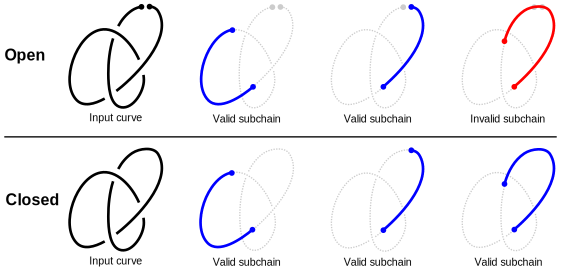
\includegraphics[width=1\textwidth]{subchains.pdf}
\caption{With open input curve (upper panel), subchains are not allowed to contain endpoints of the input curve (except at their endpoint). With closed input curve (lower panel), all subchains are allowed. Example of valid subchains are shown in blue, and invalid subchain in red. }\label{fig:subchains}
\end{figure}

With closed input curves, one should be careful when interpreting the output of \lstinline{knotted_core}. Indeed, in the output of \lstinline{knotted_core}\footnote{see section ``\ref{sec:format:listsubchains} \nameref{sec:format:listsubchains}'' for more information on the file format.}, subchains are defined by two points of the input curve (\lstinline{index_first} and \lstinline{index_last}). When the first point has an index $i_1$ lower than the last point $i_2$, the subchain consist of all points with indices: $\{i_1,i_1+1,i_1+2,\cdots,i_2\}$.
However, when the first point has an index $i_1$ higher than the last point $i_2$, the subchain consist of all points with index larger or equal to the index of the first point up to the last point of the input curve, and then continue with the first point of the input curve up to $i_2$, i.e. for an input curve with $N$ points (using zero-based indexing): $\{i_1,i_1+1,i_1+2,\cdots,N-1,0,1,2,\cdots,i_2\}$. For example, the output
\begin{lstlisting}
#index_first  index_last  length  frequency  polynomial
3             8           6      0.5       - A^(-16) + A^(-12) + A^(-4)
\end{lstlisting}
corresponds to the subchain with points $\{3,4,5,6,7,8\}$ of the input curve, while 
\begin{lstlisting}
#index_first  index_last  length  frequency  polynomial
109           3           6      0.5       - A^(-16) + A^(-12) + A^(-4)
\end{lstlisting}
corresponds to the subchain with points $\{109,110,0,1,2,3\}$ of the input curve (which has 111 points).

All options discussed when using open input curve can also be used with closed curve. In particular, the option \lstinline{--closure-method}, which defines how each subchain should be closed (or kept open), can be used independently from the choice of closure for the input curve (\lstinline{--cyclic-input}). For example, to evaluate the knotted core of the closed input curve \lstinline{examples/3_1m_supercoiled.xyz} based on the evaluation of the polynomial invariant of open subchains projected on the sphere (Jones polynomial for knotoids):
\begin{lstlisting}
$ bin/knotted_core --output-all=all.txt --output-search=search.txt --output=knotted-core.txt \
  --names-db=internal --nb-projections=100 --cyclic-input \
  examples/3_1m_supercoiled.xyz
\end{lstlisting}
The resulting knotted core is saved in the file \lstinline{knotted-core.txt}, while the dominant knotoid types of all possible subchains and of all subchains evaluated during the search are saved in files \lstinline{all.txt} and \lstinline{search.txt} respectively.


The resulting files can be used to produce a disk matrix\cite{rawdon} 
with \lstinline{plot_knotted_core.R} and option \lstinline{--cyclic} (see Figure~\ref{fig:3_1m_supercoiled:disk}):
\begin{lstlisting}
$ scripts/plot_knotted_core.R --cyclic --output=disk_matrix.png \
  --knotted-core=knotted-core.txt all.txt
\end{lstlisting}
\begin{figure}[t]
\centering
\includegraphics[width=0.9\textwidth,trim={300px 0 300px 0},clip]{3_1m_supercoiled_disk_matrix.png}
\caption{ The disk matrix of the closed curve \lstinline{examples/3_1m_supercoiled.xyz}. Radial coordinate corresponds to the length of the subchain and angular coordinate to the midpoint of the subchain. Color corresponds to dominant knotoid type of the subchain and transparency to its frequency. The knotted core is shown with a yellow circle.}\label{fig:3_1m_supercoiled:disk}
\end{figure}



\clearpage
\subsection{\label{sec:example}Real life example: protein 3KZN}
In this section we apply the concepts discussed above on a real life example.
\subsubsection{Knotoids}
We start by downloading the protein structure that we want to analyze from the Protein database (PDB)\cite{pdb}. In this example we shall use the protein 3KZN\cite{shi2006} that is known to form a deep trefoil knot.
\begin{lstlisting}
$ wget https://files.rcsb.org/download/3KZN.pdb
\end{lstlisting}
Note for Windows users: with the {\it Windows PowerShell}, \lstinline{wget} needs the additional option \lstinline{-OutFile 3KZN.pdb}. Alternatively, the file \lstinline{https://files.rcsb.org/download/3KZN.pdb} can be simply downloaded using a web browser.

The next step is to extract from the .pdb file the $xyz$-coordinates of the $C_\alpha$ atoms, that make up the protein backbone and store them into a file with xyz file format\footnote{see section ``\ref{sec:format:xyz} \nameref{sec:format:xyz}'' for more information on the file format.}. Note that a protein molecule may include more than one chains in its conformation so one has to be careful when extracting coordinates. In this example we work with chain $A$.
Note that many proteins that are deposited in the PDB have gaps in their conformations. If this is the case, the gaps are connected with a straight line. One should be careful when dealing with such situations since connecting the endpoints of a gap with a straight line may alter the topology of the chain.
For further details on the .pdb file format, the reader should refer to the documentation at \url{http://www.wwpdb.org/documentation/file-format}. The simple script \lstinline{pdb_to_xyz.R}\footnote{To use this script, {\ttfamily R}\cite{r2017} must be installed with packages {\ttfamily optparse}\cite{optparse} and {\ttfamily Rpdb}\cite{rpdb}.} distributed with {\it Knoto-ID} can be used to convert the pdb file \lstinline{3KZN.pdb} to xyz format and save the output to \lstinline{examples/3KZN_chain_A.xyz}:
\begin{lstlisting}
$ scripts/pdb_to_xyz.R --output=examples/3KZN_chain_A.xyz 3KZN.pdb
\end{lstlisting}

We can evaluate the Jones polynomial for knotoids on the sphere of this protein chain by calling the command:
\begin{lstlisting}
$ bin/polynomial_invariant examples/3KZN_chain_A.xyz 
\end{lstlisting}
which generates the following output to standard error:
\begin{lstlisting}
seed: 1501677085
polynomial invariant: Jones polynomial for knotoids.
Loading input curve
3D curve has 331 vertices
projection: -0.443782,-0.690045,-0.571748
Simplifying 3D curve
3D curve has 13 vertices
Evaluating diagram
diagram has 8 crossings
Simplifying diagram
diagram has 5 crossings
Simplifying diagram with random reidemeister moves III (max 100000 moves)
diagram has 5 crossings
Final simplifying diagram
diagram has 5 crossings
\end{lstlisting}
As we can see, the output includes information, amongst other things, on the random projection that was used and an upper bound on the crossing number of the diagram. After completion, the Jones polynomial for knotoids of the chain is written to standard output:
\begin{lstlisting}
Polynomial:  - A^(-16) + A^(-12) + A^(-4)
\end{lstlisting}
For the moment, we don't have any information on the knotoid type that corresponds to this polynomial. However, this can be solved easily by using the option \lstinline{--names-db} to specify a knotoid names database:
\begin{lstlisting}
$ bin/polynomial_invariant --projection="-0.443782,-0.690045,-0.571748" \
  --names-db=internal examples/3KZN_chain_A.xyz
\end{lstlisting}
We have used the option \lstinline{--projection} in order to use a fixed projection for our chain. In particular, we used the projection that was randomly chosen in the previous run. The option \lstinline{--names-db=internal} allows the loading of the internal knot(oid)s names database. Instead of the keyword \lstinline{internal}, an external file specifying the mapping from polynomials to names can also be given\footnote{see section ``\ref{sec:format:namesdb} \nameref{sec:format:namesdb}'' for more information on the file format.}. The standard output now takes the following form:
\begin{lstlisting}
Knotoid type: 3_1m      Polynomial:  - A^(-16) + A^(-12) + A^(-4)
\end{lstlisting}
This means that this particular projection of the protein chain corresponds to a knot-type knotoid with 3 crossings. As mentioned in section ``\ref{sec:theory} \nameref{sec:theory}'', the chain is considered lying inside a large enough sphere. Each point of the sphere indicates a projection direction towards an oriented surface that lies outside the sphere that encloses the chain. There are two options for the oriented surface: a sphere, which is the default option and is the one that was used so far in this example, as well as the 2D plane. By adding the option \lstinline{--planar}, we evaluate the knotoid type of the protein chain using planar knotoids.
\begin{lstlisting}
$ bin/polynomial_invariant --projection="-0.443782,-0.690045,-0.571748" \
  --names-db=internal --planar examples/3KZN_chain_A.xyz
\end{lstlisting}
In this case the knotoid type of the protein chain remains the same upon evaluation using planar knotoids. Indeed
\begin{lstlisting}
Knotoid type: 3_1m      Polynomial:  - A^(-16) + A^(-12) + A^(-4)
\end{lstlisting}
Note that this is not the general case. There could be protein chains that have a planar knotoid type different from the knotoid type on the sphere.

To evaluate the arrow polynomial for knotoids on the sphere instead of the Jones polynomial, use option\\
\lstinline{--arrow-polynomial}:
\begin{lstlisting}
$ bin/polynomial_invariant --projection="-0.443782,-0.690045,-0.571748" \
  --names-db=internal --arrow-polynomial examples/3KZN_chain_A.xyz
\end{lstlisting}
To evaluate the loop arrow polynomial for knotoids on the plane instead of the Turaev loop bracket polynomial, use option \lstinline{--arrow-polynomial} together with \lstinline{--planar}:
\begin{lstlisting}
$ bin/polynomial_invariant --projection="-0.443782,-0.690045,-0.571748" \
  --names-db=internal --planar --arrow-polynomial examples/3KZN_chain_A.xyz
\end{lstlisting}
In this specific example, using arrow or loop arrow polynomial gives the same result as the Jones polynomial for knotoid and Turaev loop bracket polynomial.


In the example runs that we presented so far, the results were just printed to standard output. By adding the option \lstinline{--output=FILENAME}, we can ask the program to print the results into a file. Moreover, by including \lstinline{--output-diagram=FILENAME} the program creates a separate file that contains the corresponding knotoid diagram in PD format\footnote{see section ``\ref{sec:format:pd} \nameref{sec:format:pd}'' for more information on the file format.}:
\begin{lstlisting}
$ bin/polynomial_invariant --projection="-0.443782,-0.690045,-0.571748" \
  --names-db=internal --planar --output-diagram=3KZN_diagram.txt \ 
  --output=3KZN_polynomial.txt examples/3KZN_chain_A.xyz
\end{lstlisting}
Note that option \lstinline{--output-diagram-format=gauss} can be used to output extended Gauss codes\footnote{see section ``\ref{sec:format:gauss} \nameref{sec:format:gauss}'' for more information on the file format.} instead of PD codes for the knotoid diagrams.

Up until this point, we have dealt only with a single projection of the protein chain. In order to find the dominant knotoid type of a chain, we have to consider all of its projections and, subsequently, sample them in a uniform way. By adding the option \lstinline{--nb-projections=N} the program samples ${\rm N}$ random projections with uniform distribution on the surface of the sphere. Below we give an example with 100 random projections:
\begin{lstlisting}
$ bin/polynomial_invariant --nb-projections=100 --names-db=internal \
  --planar examples/3KZN_chain_A.xyz
\end{lstlisting}
The standard output includes a histogram of frequency of appearance of knotoid types. The knotoid with the highest frequency of appearance is the dominant knotoid type of the chain:
\begin{lstlistingsmall}
#frequency knotoid_type    polynomial
0.63       3_1m                       - A^(-16) + A^(-12) + A^(-4)
0.07       UNKNOWN                    - A^(-30)*v - 2*A^(-28) - A^(-28)*v - 2*A^(-26) + A^(-26)*v + A^(-24) + ...
0.07       1_1*3_1m                   + A^(-14)*v + A^(-12) - A^(-10)*v - A^(-8) - A^(-2)*v - 1
0.04       2_4s*3_1m|2_4m*3_1m        - A^(-24)*v - 2*A^(-22) - A^(-20) + A^(-20)*v + 2*A^(-18) + A^(-16) + A^...
0.04       4_4s|4_4m                  - A^(-18) - A^(-16) + A^(-14) + 2*A^(-12) - A^(-8) + A^(-4)
0.04       2_1s*3_1m|2_1m*3_1m        + A^(-26) - 2*A^(-22) - A^(-20) + A^(-18) + A^(-16) - A^(-14) + A^(-10) ...
0.03       2_6*3_1m                   + A^(-20) - A^(-16) - A^(-16)*v^(2) - A^(-14)*v + A^(-12)*v^(2) + A^(-10...
0.02       UNKNOWN                    + A^(-22) + A^(-20) + A^(-20)*v + A^(-18)*v - A^(-16) - A^(-16)*v - A^(-...
0.01       UNKNOWN                    - A^(-14) - A^(-12) - A^(-12)*v - A^(-10) - A^(-10)*v + A^(-8)*v + 2*A^(...
0.01       UNKNOWN                    - A^(-14) - A^(-12) + 2*A^(-8) + 2*A^(-6) - A^(-2)
0.01       4_46|4_46ms                - A^(-12) - A^(-10) - A^(-10)*v + A^(-6) + A^(-6)*v + A^(-4) - A^(-2)*v - 1
0.01       2_1*3_1m|2_1ms*3_1m        - A^(-12) - A^(-10) + A^(-8) + 2*A^(-6) - A^(-2) + 1 + A^(2) - A^(6)
0.01       5_81|5_81ms|5_316|5_316ms  - A^(-10) + A^(-6) - A^(-2) - A^(-2)*v - 1 - v - A^(2)
0.01       2_5*3_1m                   + A^(-14)*v - 2*A^(-10)*v - A^(-8) + A^(-6)*v + A^(-4) - A^(-2)*v + A^(2...
\end{lstlistingsmall}
In this example, the dominant knotoid type for the protein 3KZN is the knot-type knotoid $3_1m$ with frequency of appearance 63\%. Note that the exact frequency may change depending on the 100 random projections chosen. If multiple knotoid types have the same polynomial invariant\footnote{in the knotoid names database specified with \lstinline{--names-db}.}, all knotoid types are concatenated with a \lstinline{|} separator. \lstinline{UNKNOWN} corresponds to knotoids not found in the database (more than 5 crossings).

We can also use a predetermined list of projections. In the following example we use the option \lstinline{--projections-list} in order to specify a list of 100 fixed projection directions uniformly distributed on the surface of a sphere, weighted by the surface of their corresponding Voronoi cells\footnote{see section ``\ref{sec:format:projections} \nameref{sec:format:projections}'' for a description of the file format.}. 
\begin{lstlisting}
$ bin/polynomial_invariant --projections-list=examples/projections_list_100.txt \
  --names-db=internal --planar examples/3KZN_chain_A.xyz
\end{lstlisting}

Using option \lstinline{--output-diagram=diagrams.txt}, the list of projection directions with corresponding polynomials and knotoid types is saved to file \lstinline{diagrams.txt}. Although 100 projection can be sufficient to obtain a first approximation of the projection map, better results can be achieved using a larger number of projections:
\begin{lstlisting}
$ bin/polynomial_invariant --nb-projections=10000 --names-db=internal \
  --planar --output-diagram=diagrams.txt examples/3KZN_chain_A.xyz
\end{lstlisting}
The script \lstinline{plot_projection_map.R} can then be used to plot the projection map using voronoi tesselation:
\begin{lstlisting}
$ scripts/plot_projection_map.R --output=projection_map.png diagrams.txt
\end{lstlisting}
The resulting projection map is shown in Figure~\ref{fig:3KZN:projectionmap}.
\begin{figure}[t]
\centering
\includegraphics[width=1\textwidth]{3KZN_projection_map.png}
\caption{Projection map for the protein 3KZN (obtained with 10000 projections).  For a projection direction $(x,y,z)$, longitude ($\lambda$) and latitude ($\delta$) are defined as $x=\cos(\delta)\cos(\lambda)$, $y=\cos(\delta)\sin(\lambda)$, $z=\sin(\delta)$. Colors correspond to planar knotoid types. Since the voronoi tesselation is performed on the sphere, voronoi facets are separated by arcs of great circles, which do not correspond to straight line after equirectangular projection.}\label{fig:3KZN:projectionmap}
\end{figure}
The script \lstinline{plot_projection_map.R} can also be used to create a 3D globe (webGL) with the backbone of the protein using options \lstinline{--output-3D} and \lstinline{--curve-3D}:
\begin{lstlisting}
$ scripts/plot_projection_map.R --output=projection_map.png --output-3D=projection_map.html \
  --curve-3D=examples/3KZN_chain_A.xyz diagrams.txt
\end{lstlisting}
A screenshot is shown in Figure~\ref{fig:3KZN:projectionmap:3D}.
\begin{figure}[t]
\centering
\includegraphics[width=1\textwidth]{3KZN_projection_map_3D.png}
\caption{3D projection map and backbone of the protein 3KZN, generated with the script \lstinline{plot_projection_map.R} using 10000 projections. Color corresponds to polynomial.}\label{fig:3KZN:projectionmap:3D}
\end{figure}


\subsubsection{Knots}
In order to analyze an open protein chain using knots, one works in an analogous way. Since the protein chain is an open 3D curve, we have to specify what method should be used to close the curve. At the moment the program supports two closure methods: ``direct'' and ``rays''\footnote{more details on these methods can be found in section ``\ref{sec:theory:knotoidsandcurves} \nameref{sec:theory:knotoidsandcurves}''.}. These can be specified by adding the option \lstinline{--closure-method=direct} for the former and \lstinline{--closure-method=rays} for the latter.
\begin{lstlisting}
$ bin/polynomial_invariant --closure-method=rays --names-db=internal \
  examples/3KZN_chain_A.xyz
\end{lstlisting}

The choice of projection directions can be specified with \lstinline{--nb-projections} or \lstinline{--projections-list} as discussed above. However, since the \lstinline{direct} closure (\lstinline{--closure-method=direct}) does not depend on the direction of projection, using multiple projections should only be used with \lstinline{--closure-method=rays}.

\subsubsection{Subchains, knotted cores and fingerprint matrices}
We would like now to analyze the subchains of 3KZN's backbone using the \lstinline{knotted_core} program. We start by calling
\begin{lstlisting}
$ bin/knotted_core examples/3KZN_chain_A.xyz 
\end{lstlisting}
The program will search for the knotted core, which is the shortest subchain obtained by progressively altering the length of the input curve by 1 point without changing the dominant knotoid type in the process. The dominant knotoid type of each subchain is evaluated by projecting on a sphere (using \lstinline{--nb-projections=20} by default). During the run, information on the progression will be written to standard error and after completion, the knotted core will be written to standard output
\begin{lstlisting}
#index_first  index_last  length  frequency  polynomial
168           252         85      0.5        - A^(-16) + A^(-12) + A^(-4)
170           254         85      0.45       - A^(-16) + A^(-12) + A^(-4)
\end{lstlisting}
Each line corresponds to a possible knotted core. Here, two subchains have the same the minimal length. Note that this list of possible knotted cores may change due to the random sampling of the 20 projection directions. The first knotted core is the subchain with starting index 168 (using zero-based indexing) and ending index 252 and it has a dominant polynomial invariant $-A^{-16}+A^{-12}+A^{-4}$ that appears in 50\% of the projections\footnote{see section ``\ref{sec:format:listsubchains} \nameref{sec:format:listsubchains}'' for more information on the file format.}. The second solution starts at index 170, ends at index 254 and has the same dominant polynomial invariant that appears in 45\% of the projection.

In analogy with the case explained above, we can specify the number of random projections that we want our sample to include (\lstinline{--nb-projections} or \lstinline{--projections-list}), the knot or knotoid names (\lstinline{--names-db}), the option of evaluating the diagrams on the plane (\lstinline{--planar}), the closure method (\lstinline{--closure-method}) and so on. For example, the following finds the knotted core of 3KZN using a set of predetermined projection directions and also loads the knotoid names database:
\begin{lstlisting}
$ bin/knotted_core --projections-list=examples/projections_list_100.txt \
  --names-db=internal examples/3KZN_chain_A.xyz
\end{lstlisting}
When the option \lstinline{--names-db} is used, the output has an additional column with the knot(oid) type corresponding to the dominant polynomial invariant (here 3\_1m):
\begin{lstlisting}
#index_first  index_last  length  frequency  knotoid_type  polynomial
170           252         83      0.260337   3_1m          - A^(-16) + A^(-12) + A^(-4)
\end{lstlisting}



We proceed and ask \lstinline{knotted_core} to produce all data required to generate the fingerprint matrix of 3KZN (using options \lstinline{--output-all}, \lstinline{--output-search} and \lstinline{--output}). WARNING: evaluating all subchains (option \lstinline{--output-all}) can be very slow\footnote{On a MacBook Pro from 2011 with 2.4 GHz Intel Core i5 CPU, it takes approximately 15 minutes to execute this command.}.
\begin{lstlisting}
$ bin/knotted_core --names-db=internal \
  --output-all=3KZN_all.txt --output-search=3KZN_search.txt \
  --output=3KZN_knotted_core.txt --timeout=1 examples/3KZN_chain_A.xyz
\end{lstlisting}
The option \lstinline{--timeout=1} was used to interrupt the evaluation of the polynomial after 1 second. Indeed, for a few subchains and projections, the resulting diagram has a large number of crossings and the evaluation of the polynomial invariant may be very slow. Note that if the evaluation of a polynomial invariant takes more than 1 second, the knot type and polynomial invariant are set to \lstinline{TIMEOUT}. This special value is treated as any other polynomial invariant and knot type and will appear in the output if it is the dominant knot type.

Subsequently we call the {\ttfamily R} script that creates the fingerprint matrix:
\begin{lstlisting}
$ scripts/plot_knotted_core.R --output=3KZN_fingerprint_matrix.png 3KZN_all.txt
\end{lstlisting}
To overlay the knotted core(s) (yellow circle):
\begin{lstlisting}
$ scripts/plot_knotted_core.R --output=3KZN_fingerprint_matrix.png \
  --knotted-core=3KZN_knotted_core.txt 3KZN_all.txt 
\end{lstlisting}
The resulting fingerprint matrix is shown in Figure~\ref{fig:3KZN:fingerprint}.
\begin{figure}[t]
\centering
\includegraphics[width=0.9\textwidth,trim={200px 0 250px 0},clip]{3KZN_fingerprint_matrix.png}
\caption{The knotoid fingerprint matrix for the protein 3KZN. This proteins forms a deep trefoil knotoid (bottom left corner corresponds to the full chain). Color corresponds to dominant knotoid type of the subchain and transparency corresponds to its frequency. Yellow circles are centered on knotted core(s).}\label{fig:3KZN:fingerprint}
\end{figure}
The fingerprint matrix is dominated by 0\_1, 2\_1m and 3\_1m knotoids. However, because of the random sampling of a small number of projection directions used to estimate the dominant knotoid type (\lstinline{--nb-projections=20} by default), the figure has a high level of noise and several other knotoid types appear in the regions where the frequency of the dominant knotoid type is low. To decrease the level of noise, one possibility is to increase the number of projections. Figure~\ref{fig:3KZN:fingerprint1000} presents the same fingerprint matrix as in Figure~\ref{fig:3KZN:fingerprint} but obtained with \lstinline{--nb-projections=1000}. As expected, increasing the number of projections strongly decreases the level of noise, and only three dominant knotoid types remain (0\_1, 2\_1m and 3\_1m). In addition, a unique and shorter knotted core could be found (starting index 170, ending index 253, appearing in 31\% of the projections).
Obviously, increasing the number of projection not only increases the accuracy of the resulting fingerprint matrix, but it also increases the computational cost, which can quickly become prohibitively high. Therefore, it may be worth keeping the number of projection low to obtain a first approximation of the fingerprint matrix, which may be sufficient for most applications (compare Figure~\ref{fig:3KZN:fingerprint} and Figure~\ref{fig:3KZN:fingerprint1000}). 
\begin{figure}[t]
\centering
\includegraphics[width=0.9\textwidth,trim={200px 0 250px 0},clip]{3KZN_fingerprint_matrix_1000.png}
\caption{The knotoid fingerprint matrix for the protein 3KZN obtained with \lstinline{--nb-projections=1000}. A yellow circle is centered on the knotted core.}\label{fig:3KZN:fingerprint1000}
\end{figure}

Finally, we ask \lstinline{knotted_core} to produce the disk matrix of 3KZN. Since the endpoints of the chain are very close, there is no problem with connecting them with a straight line and to consider the input curve as circular (option \lstinline{--cyclic-input}). In addition, we ask \lstinline{knotted_core} to close each subchain with the \lstinline{rays} closure method\footnote{see section ``\ref{sec:theory:knotoidsandcurves} \nameref{sec:theory:knotoidsandcurves}'' for more details.}. Please note that the closure method for the input curve (option \lstinline{--cyclic-input}) and for the subchains (\lstinline{--closure-method}) can be chosen independently. WARNING: evaluating all subchains (option \lstinline{--output-all}) can be very slow\footnote{On a MacBook Pro from 2011 with 2.4 GHz Intel Core i5 CPU, it takes approximately 50 minutes to execute this command.}.
\begin{lstlisting}
$ bin/knotted_core --cyclic-input --closure-method=rays --names-db=internal \
  --output-all=3KZN_all.txt --output-search=3KZN_search.txt \
  --output=3KZN_knotted_core.txt --timeout=1 examples/3KZN_chain_A.xyz
\end{lstlisting}

A disk matrix can be produced using \lstinline{plot_knotted_core.R} with option \lstinline{--cyclic}.  WARNING: drawing heatmaps in polar coordinate using {\ttfamily R} package {\ttfamily ggplot2}\cite{wickham2009} can be very slow\footnote{On a MacBook Pro from 2011 with 2.4 GHz Intel Core i5 CPU, it takes approximately 20 minutes to execute this command.}.
\begin{lstlisting}
$ scripts/plot_knotted_core.R --cyclic --output=3KZN_circular_matrix.png \
  --knotted-core=3KZN_knotted_core.txt 3KZN_all.txt
\end{lstlisting}
The resulting disk matrix is shown in Figure~\ref{fig:3KZN:disk}
\begin{figure}[t]
\centering
\includegraphics[width=0.9\textwidth,trim={280px 0 300px 0},clip]{3KZN_circular_matrix.png}
\caption{The disk matrix for the protein 3KZN with uniform closure (i.e. \lstinline{--closure-method=rays} in multiple directions). This proteins forms a right handed trefoil knot (all points on the enclosing circle corresponds to the full chain). Color corresponds to dominant knot type of the subchain and transparency corresponds to its frequency. Yellow circles are centered around knotted core(s).}\label{fig:3KZN:disk}
\end{figure}



\clearpage

% Copyright (C) 2017 by SIB Swiss Institute of Bioinformatics, Julien Dorier and Dimos Goundaroulis.
% 
% This file is part of project Knoto-ID.
% 
% Knoto-ID is free software: you can redistribute it and/or modify
% it under the terms of the GNU General Public License as published by
% the Free Software Foundation, either version 2 of the License, or
% (at your option) any later version.
% 
% Knoto-ID is distributed in the hope that it will be useful,
% but WITHOUT ANY WARRANTY; without even the implied warranty of
% MERCHANTABILITY or FITNESS FOR A PARTICULAR PURPOSE.  See the
% GNU General Public License for more details.
% 
% You should have received a copy of the GNU General Public License
% along with Knoto-ID.  If not, see <http://www.gnu.org/licenses/>.

\section{\label{sec:reference}Command reference}

\subsection{Polynomial invariant}
\subsubsection{Usage}
\begin{lstlisting}
$ bin/polynomial_invariant [options] FILENAME
\end{lstlisting}

Load a piecewise linear curve from file  \lstinline{FILENAME}\footnote{in xyz file format, see section ``\ref{sec:format:xyz} \nameref{sec:format:xyz}'' for more information on the file format.}. To read from standard input instead, use file name \lstinline{stdin} or \lstinline{-}. By default, the curve is open (knotoid), but it can be closed (knot) by specifying a closure method with option \lstinline{--closure-method}. 
The input curve is then simplified using a 3D triangle elimination method\footnote{see section  ``\ref{sec:algorithms:3dsimplication} \nameref{sec:algorithms:3dsimplication}'' for more details.}.

Evaluate the knot(oid) diagram obtained by projecting the curve along  a randomly chosen projection direction (with uniform distribution on the surface of the sphere) or along the direction specified with option \lstinline{--projection}.
Alternatively, if \lstinline{--input-format=pd} or \lstinline{--input-format=gauss}, load directly the PD or extended Gauss code for a knot(oid) diagram from file \lstinline{FILENAME}.

Check that the knot(oid) diagram is valid using the method proposed by Vijayan and Wigderson\cite{Vijayan1982}.

Simplify the knot(oid) diagram with  Reidemeister moves\footnote{see section  ``\ref{sec:algorithms:diagramsimplication} \nameref{sec:algorithms:diagramsimplication}'' for more details.}.

Evaluate the polynomial invariant for the knot(oid) diagram on the surface of a sphere (by default) or on a plane (with option \lstinline{--planar}).

Output the polynomial invariant, and optionally the knot(oid) diagram\footnote{Output the simplified diagram.} (with option \lstinline{--output-diagram}).

If options \lstinline{--nb-projections} or  \lstinline{--projections-list} are used, the above procedure is repeated for all projections, and the output is a distribution of polynomials.

The polynomial invariant is the classical Jones polynomial for knots\cite{jones} when the curve in closed\\
(\lstinline{--closure-method=direct} or \lstinline{rays}), the Jones polynomial for knotoids\cite{turaev,guka} when the curve is open and the knotoid diagram is on the surface of a sphere (\lstinline{--closure-method=open}, without \lstinline{--planar}), and the Turaev loop bracket polynomial for knotoid\cite{turaev}  when the curve is open and the knotoid diagram is on the surface of a plane (\lstinline{--closure-method=open} and \lstinline{--planar}).


\subsubsection{Options}
\begin{description}
\item[\lstinline{-h}, \lstinline{--help}]\hfill\\
  Print usage.
\item[\lstinline{-V}, \lstinline{--version}]\hfill\\
  Print {\it Knoto-ID} version.
\item[\lstinline{-s SEED}, \lstinline{--seed=SEED}]\hfill\\
  Initialize the random number generator with  seed \lstinline{SEED}. If not specified, the seed is taken from the current time. 
\item[\lstinline{-F FORMAT}, \lstinline{--input-format=FORMAT}]\hfill\\
  Specify input format. Possible values for \lstinline{FORMAT}:
  \begin{itemize}
    \item \lstinline{xyz} piecewise linear curve in xyz file format\footnote{see section ``\ref{sec:format:xyz} \nameref{sec:format:xyz}'' for more information on the file format.}.
    \item \lstinline{pd} PD code for a knot(oid) diagram in KnotTheory file format\footnote{see section ``\ref{sec:format:pd} \nameref{sec:format:pd}''  for more information on the file format.}.  With input format \lstinline{pd}, options \lstinline{--projection}, \lstinline{--nb-projections}, \lstinline{--projections-list} and  \lstinline{--closure-method} are ignored. 
    \item \lstinline{gauss} extended Gauss code for a knot(oid) diagram\footnote{see section ``\ref{sec:format:gauss} \nameref{sec:format:gauss}''  for more information on the file format.}. Use option \lstinline{--closure-method=open} to specify that the diagram is open and \lstinline{--closure-method=direct} or \lstinline{rays} to specify that the diagram is  closed. With input format \lstinline{gauss}, options \lstinline{--projection}, \lstinline{--nb-projections} and \lstinline{--projections-list} are ignored. 
  \end{itemize}
  Default: \lstinline{xyz}.
\item[\lstinline{-o FILENAME}, \lstinline{--output=FILENAME}]\hfill\\
  Output the polynomial or distribution of polynomials to file \lstinline{FILENAME}.  To write to standard output, use file name \lstinline{stdout} or \lstinline{-}.\\
  Default \lstinline{stdout}.
\item[\lstinline{--output-diagram=FILENAME}]\hfill\\
  Output the knot(oid) diagram or list diagrams to  file \lstinline{FILENAME} using format specified with \lstinline{--output-diagram-format}. To write to standard output, use file name \lstinline{stdout} or \lstinline{-}.
\item[\lstinline{--output-diagram-format=FORMAT}]\hfill\\
  Specify output format for knot(oid) diagrams. Possible values for \lstinline{FORMAT}:
  \begin{itemize}
    \item \lstinline{pd} PD code for a knot(oid) diagram in KnotTheory file format\footnote{see section ``\ref{sec:format:pd} \nameref{sec:format:pd}''  for more information on the file format.}.  
    \item \lstinline{gauss} extended Gauss code for a knot(oid) diagram\footnote{see section ``\ref{sec:format:gauss} \nameref{sec:format:gauss}''  for more information on the file format.}.
  \end{itemize}
  Default: \lstinline{pd}.
\item[\lstinline{-m METHOD}, \lstinline{--closure-method=METHOD}]\hfill\\
  Specify how to close the input curve. Possible values for \lstinline{METHOD}:
  \begin{itemize}
  \item \lstinline{open} the curve is open (knotoid).
  \item \lstinline{direct} connect last point to first point by a straight line.
  \item \lstinline{rays} close by extending two parallel rays along the projection direction, each originating from one of the endpoints of the curve and connecting them outside the sphere that encloses the curve\footnote{see section ``\ref{sec:theory:knotoidsandcurves} \nameref{sec:theory:knotoidsandcurves}'' for more details.}.
  \end{itemize}
  Default: \lstinline{open}.
\item[\lstinline{-p}, \lstinline{--planar}]\hfill\\
  Evaluate polynomial invariant for the knot(oid) diagram on a plane. If not specified, evaluate polynomial invariant for the knot(oid) diagram on the surface of a sphere. This option is only relevant for open curves (\lstinline{--closure-method=open}).
\item[\lstinline{--nb-moves-III=NMOVES}]\hfill\\
  Use \lstinline{NMOVES} iterations to simplify the knot(oid) diagram using Reidemeister move III\footnote{see section  ``\ref{sec:algorithms:diagramsimplication} \nameref{sec:algorithms:diagramsimplication}'' for more details.}.\\
  Default \lstinline{100000}.
\item[\lstinline{--projection="X,Y,Z"}]\hfill\\ Project the input curve along projection direction (X,Y,Z). If not specified, use randomly chosen projection direction (with uniform distribution on the surface of the sphere).
\item[\lstinline{-N NPROJ}, \lstinline{--nb-projections=NPROJ}]\hfill\\
  Choose \lstinline{NPROJ} random projection directions (with uniform distribution on the surface of the sphere) and evaluate the corresponding polynomial invariant for each projection. Note:
  \begin{itemize}
  \item Instead of a unique polynomial, the output specified with \lstinline{--output} will contain the distribution of polynomials\footnote{see section ``\ref{sec:format:multiprojection:jones} \nameref{sec:format:multiprojection:jones}'' for more information on the file format.}. 
    \item The output specified with \lstinline{--output-diagram} will contain a list of projections with polynomials and knot(oid) diagrams\footnote{see section ``\ref{sec:format:multiprojection:diagrams} \nameref{sec:format:multiprojection:diagrams}'' for more information on the file format.}.
    \item For cyclic curves with closure method \lstinline{direct} the polynomial invariant (classical Jones polynomial) does not depend on the projection. To avoid useless computations \lstinline{NPROJ} will be set to 1.
    \item Option \lstinline{--projection} is ignored.                                  
  \end{itemize}
\item[\lstinline{--projections-list=FILENAME}]\hfill\\
  Load a list of projection directions from \lstinline{FILENAME}\footnote{see section ``\ref{sec:format:projections} \nameref{sec:format:projections}'' for more information on the file format.} and evaluate the corresponding polynomial invariant for each projection. Note:
  \begin{itemize}
  \item Instead of a unique polynomial, the output specified with \lstinline{--output} will contain the distribution of polynomials\footnote{see section ``\ref{sec:format:multiprojection:jones} \nameref{sec:format:multiprojection:jones}'' for more information on the file format.}. 
    \item The output specified with \lstinline{--output-diagram} will contain a list of projections with polynomials and knot(oid) diagrams\footnote{see section ``\ref{sec:format:multiprojection:diagrams} \nameref{sec:format:multiprojection:diagrams}'' for more information on the file format.}.
    \item For cyclic curves with closure method \lstinline{direct} the polynomial invariant (classical Jones polynomial) does not depend on the projection. To avoid useless computations, only one projection direction will be used.
    \item Options  \lstinline{--nb-projections} and \lstinline{--projection} are ignored.                                  
  \end{itemize}
\item[\lstinline{-n FILENAME}, \lstinline{--names-db=FILENAME}]\hfill\\
  Load a list of polynomials with corresponding knot(oid) names from file \lstinline{FILENAME}\footnote{see section ``\ref{sec:format:namesdb} \nameref{sec:format:namesdb}'' for more information on the file format.}.
\item[\lstinline{--timeout=TIMEOUT}]\hfill\\
  Abort evaluation of polynomial invariant after \lstinline{TIMEOUT} seconds (integer number). Note: if the evaluation of the polynomial invariant is aborted, the polynomial is replaced by \lstinline{TIMEOUT}.
\end{description}


      
\subsection{Knotted core}
\subsubsection{Usage}
\begin{lstlisting}
$ bin/knotted_core [options] FILENAME
\end{lstlisting}

Load a piecewise linear curve from file  \lstinline{FILENAME}\footnote{in xyz file format, see section ``\ref{sec:format:xyz} \nameref{sec:format:xyz}''  for more information on the file format.} and evaluate the knotted core\footnote{see section  ``\ref{sec:algorithms:knottedcore} \nameref{sec:algorithms:knottedcore}'' for more information on the file format.}.
To read from standard input instead, use file name \lstinline{stdin} or \lstinline{-}.
By default, the curve is considered open, but it can be closed with option \lstinline{--cyclic-input}.

Output the knotted core,  and optionally all subchains tested when searching the knotted core (with option \lstinline{--output-search}) as well as all possible subchains of the input curve (with option \lstinline{--output-all}).

Note that the knotted core corresponds to the "top-down" knotted core discussed by Tubiana and coauthors \cite{tubiana2011}.

\subsubsection{Options}
\begin{description}
\item[\lstinline{-h}, \lstinline{--help}]\hfill\\
  Print usage.
\item[\lstinline{-V}, \lstinline{--version}]\hfill\\
  Print {\it Knoto-ID} version.
\item[\lstinline{-s SEED}, \lstinline{--seed=SEED}]\hfill\\
  Initialize the random number generator with  seed \lstinline{SEED}. If not specified, the seed is taken from the current time. 
\item[\lstinline{-o FILENAME}, \lstinline{--output=FILENAME}]\hfill\\
  Output the knotted core to file \lstinline{FILENAME}\footnote{see section ``\ref{sec:format:listsubchains} \nameref{sec:format:listsubchains}'' for more information on the file format.}.  To write to standard output, use file name \lstinline{stdout} or \lstinline{-}.\\
  Default \lstinline{stdout}.
\item[\lstinline{--output-search=FILENAME}]\hfill\\
  Output all subchains tested when searching for the knotted core to file \lstinline{FILENAME}\footnote{see section ``\ref{sec:format:listsubchains} \nameref{sec:format:listsubchains}'' for more information on the file format.}. To write to standard output, use file name \lstinline{stdout} or \lstinline{-}.
\item[\lstinline{--output-all=FILENAME}]\hfill\\
  Output all possible subchains of the input curve to file \lstinline{FILENAME}\footnote{see section ``\ref{sec:format:listsubchains} \nameref{sec:format:listsubchains}'' for more information on the file format.}. To write to standard output, use file name \lstinline{stdout} or \lstinline{-}. Warning: evaluating the polynomial invariants for all subchains of the input curve may be slow.
\item[\lstinline{-C}, \lstinline{--cyclic-input}]\hfill\\
  Close the input curve by connecting its last point to its first point by a straight line.  
\item[\lstinline{-m METHOD}, \lstinline{--closure-method=METHOD}]\hfill\\
  Specify how to close each subchain. Possible values for \lstinline{METHOD}:
  \begin{itemize}
  \item \lstinline{open} the subchain is open (knotoid).
  \item \lstinline{direct} connect last point to first point by a straight line.
  \item \lstinline{rays} close by extending two parallel rays along the projection direction, each originating from one of the endpoints of the curve and connecting them outside the sphere that encloses the curve\footnote{see section ``\ref{sec:theory:knotoidsandcurves} \nameref{sec:theory:knotoidsandcurves}'' for more details.}.
  \end{itemize}
  Default: \lstinline{open}.
\item[\lstinline{-p}, \lstinline{--planar}]\hfill\\
  For each subchain, evaluate its polynomial invariant for the knot(oid) diagram on a plane. If not specified, evaluate polynomial invariant for the knot(oid) diagram on the surface of a sphere. This option is only relevant for open curves (\lstinline{--closure-method=open}).
\item[\lstinline{--nb-moves-III=NMOVES}]\hfill\\
  Use \lstinline{NMOVES} iterations to simplify the knot(oid) diagram using Reidemeister move III\footnote{see section  ``\ref{sec:algorithms:diagramsimplication} \nameref{sec:algorithms:diagramsimplication}'' for more details.}.\\
  Default \lstinline{10}.
\item[\lstinline{-N NPROJ}, \lstinline{--nb-projections=NPROJ}]\hfill\\
  Use \lstinline{NPROJ} random projection directions (with uniform distribution on the surface of the sphere) to evaluate the dominant polynomial invariant of each subchain.  For cyclic subchains with closure method \lstinline{direct} the polynomial invariant (classical Jones polynomial) does not depend on the projection. To avoid useless computations \lstinline{NPROJ} will be set to 1.\\
  Default: \lstinline{20}.
\item[\lstinline{--projections-list=FILENAME}]\hfill\\
 Evaluate the dominant polynomial using the list of projection directions in file \lstinline{FILENAME}\footnote{see section ``\ref{sec:format:projections} \nameref{sec:format:projections}''  for more information on the file format.}. Note:
  \begin{itemize}
    \item For cyclic subchains with closure method \lstinline{direct} the polynomial invariant (classical Jones polynomial) does not depend on the projection. To avoid useless computations, only one projection direction will be used.
    \item Options  \lstinline{--nb-projections} is ignored.                                  
  \end{itemize}
\item[\lstinline{-n FILENAME}, \lstinline{--names-db=FILENAME}]\hfill\\
  Load a list of polynomials with corresponding knot(oid) names from file \lstinline{FILENAME}\footnote{see section ``\ref{sec:format:namesdb} \nameref{sec:format:namesdb}'' for more information on the file format.}.
\item[\lstinline{--timeout=TIMEOUT}]\hfill\\
  Abort evaluation of polynomial invariant after \lstinline{TIMEOUT} seconds (integer number). Note: if the evaluation of the polynomial invariant is aborted, the polynomial is replaced by \lstinline{TIMEOUT}.
\end{description}

\subsection{Convert diagram}
\subsubsection{Usage}
\begin{lstlisting}
$ bin/convert_diagram [options] FILENAME
\end{lstlisting}


Load a knot(oid) diagram file \lstinline{FILENAME}. To read from standard input instead, use file name \lstinline{stdin} or \lstinline{-}.

Depending on \lstinline{--input-format}, different types of files can be opened:
\begin{itemize}
\item If  \lstinline{--input-format=pd} (by default), load the diagram in PD code format \footnote{see section ``\ref{sec:format:pd} \nameref{sec:format:pd}''  for more information on the file format.}.
\item If  \lstinline{--input-format=gauss}, load the diagram in extended Gauss code format\footnote{see section ``\ref{sec:format:gauss} \nameref{sec:format:gauss}''  for more information on the file format.}. Option \lstinline{--closure-method} is used to specify whether the diagram is open (default) or closed.
\item If  \lstinline{--input-format=xyz}, load a piecewise linear curve in xyz format\footnote{see section ``\ref{sec:format:xyz} \nameref{sec:format:xyz}'' for more information on the file format.}. 
  By default, the curve is open (knotoid), but it can be closed (knot) by specifying a closure method with option \lstinline{--closure-method}.
  If option \lstinline{--3D-reduction} is given, the input curve is simplified using a 3D triangle elimination method\footnote{see section  ``\ref{sec:algorithms:3dsimplication} \nameref{sec:algorithms:3dsimplication}'' for more details.}.
  
  A knot(oid) diagram is then obtained by projecting the curve along a randomly chosen projection direction (with uniform distribution on
  the surface of the sphere) or along the direction specified with  option \lstinline{--projection}.  
\end{itemize}
Check that the knot(oid) diagram is valid using the method proposed by Vijayan and Wigderson\cite{Vijayan1982}.


If option \lstinline{--simplify-diagram} is given, the knot(oid) diagram is simplified using Reidemeister moves.
Finally, the resulting diagram is saved to file specified by option \lstinline{--output}, with format specified by \lstinline{--output-format}.

Notes:
\begin{itemize}
\item If the input is in xyz format or contains information on which arcs
  touch the outside region, option \lstinline{--planar} can be used to keep this information 
  in the output.
\item To output in ``xyz for knot(oid) diagram`` format, \lstinline{convert_diagram} uses a circle packing algorithm\footnote{see section ``\ref{sec:algorithms:circlepacking} \nameref{sec:algorithms:circlepacking}'' for more information.} to draw the diagram in the x-y plane (with z storing information on what stand is above/below in each crossing). While this algorithm usually produces good results for knot diagrams (see Figures \ref{fig:diagram1} and \ref{fig:diagram2}), it may also produce poorly balanced results, with circle radii (or arc lengths) differing by several orders of magnitude. This problem of unbalanced circle packing is particularly strong for planar knotoid diagrams, in particular when the diagram is enclosed within an external loop. To mitigate this problem, it is possible to use a simulated annealing algorithm to ``relax'' the diagram (with option \lstinline{--nb-iterations-relaxation}).
  By default, if the resulting diagram is not balanced (i.e. ratio of largest arc length to shortest arc length is larger than 20), \lstinline{convert_diagram} will quit with an error without writing the resulting diagram (to avoid producing unreadable and potentially misleading output). To ignore this test and write the diagram even if it is unbalanced, use option \lstinline{--force}.
\end{itemize}


\subsubsection{Options}
\begin{description}
\item[\lstinline{-h}, \lstinline{--help}]\hfill\\
  Print usage.
\item[\lstinline{-V}, \lstinline{--version}]\hfill\\
  Print {\it Knoto-ID} version.
\item[\lstinline{-s SEED}, \lstinline{--seed=SEED}]\hfill\\
  Initialize the random number generator with  seed \lstinline{SEED}. If not specified, the seed is taken from the current time. 
\item[\lstinline{-p}, \lstinline{--planar}]\hfill\\
  Use information on what arcs are touching the outside region.
  
  WARNING: exit with error if the input file does not contain this information.
\item[\lstinline{-F FORMAT}, \lstinline{--input-format=FORMAT}]\hfill\\
  Specify input format. Possible values for \lstinline{FORMAT}:
  \begin{itemize}
  \item \lstinline{xyz} piecewise linear curve in xyz file format\footnote{see section ``\ref{sec:format:xyz} \nameref{sec:format:xyz}'' for more information on the file format.}.
  \item \lstinline{pd} PD code for a knot(oid) diagram in KnotTheory file format\footnote{see section ``\ref{sec:format:pd} \nameref{sec:format:pd}''  for more information on the file format.}.  With input format \lstinline{pd}, options \lstinline{--projection} and  \lstinline{--closure-method} are ignored. 
    If the input file contains multiple PD codes, only the first one will be used.
  \item \lstinline{gauss} extended Gauss code for a knot(oid) diagram\footnote{see section ``\ref{sec:format:gauss} \nameref{sec:format:gauss}''  for more information on the file format.}. Use option \lstinline{--closure-method=open} to specify that the diagram is open and \lstinline{--closure-method=direct} or \lstinline{rays} to specify that the diagram is closed. With input format \lstinline{gauss}, option \lstinline{--projection} is ignored.
    If the input file contains multiple Gauss codes, only the first one will be used.
  \end{itemize}
  Default: \lstinline{xyz}.
\item[\lstinline{--output-format=FORMAT}]\hfill\\
  Specify output format. Possible values for \lstinline{FORMAT}:
  \begin{itemize}
  \item \lstinline{pd} PD code for knot(oid) diagrams\footnote{see section ``\ref{sec:format:pd} \nameref{sec:format:pd}''  for more information on the file format.}. 
  \item \lstinline{gauss} extended Gauss code for knot(oid) diagrams\footnote{see section ``\ref{sec:format:gauss} \nameref{sec:format:gauss}''  for more information on the file format.}.
  \item \lstinline{xyz} xyz format for knot(oid) diagrams\footnote{see section ``\ref{sec:format:xyzdiagrams} \nameref{sec:format:xyzdiagrams}'' for more information on the file format.}.
  \end{itemize}
  Default: \lstinline{pd}.
\item[\lstinline{-o FILENAME}, \lstinline{--output=FILENAME}]\hfill\\
  Output the knot(oid) diagram to file \lstinline{FILENAME} using format specified with \lstinline{--output-format}.  To write to standard output, use file name \lstinline{stdout} or \lstinline{-}.\\
  Default \lstinline{stdout}.
  %options for diagram simplification
\item[\lstinline{--simplify-diagram}]\hfill\\
  Simplify the knot(oid) diagram using Reidemeister moves.
\item[\lstinline{--nb-moves-III=NMOVES}]\hfill\\
  Use \lstinline{NMOVES} iterations to simplify the knot(oid) diagram using Reidemeister move III\footnote{see section  ``\ref{sec:algorithms:diagramsimplication} \nameref{sec:algorithms:diagramsimplication}'' for more details.}.\\
  Default \lstinline{100000}.
  %options for xyz input format
\end{description}
\paragraph{Options for xyz input format:}
\begin{description}
\item[\lstinline{-m METHOD}, \lstinline{--closure-method=METHOD}]\hfill\\
  Specify how to close the input curve. Possible values for \lstinline{METHOD}:
  \begin{itemize}
  \item \lstinline{open} the curve is open (knotoid).
  \item \lstinline{direct} connect last point to first point by a straight line.
  \item \lstinline{rays} close by extending two parallel rays along the projection direction, each originating from one of the endpoints of the curve and connecting them outside the sphere that encloses the curve\footnote{see section ``\ref{sec:theory:knotoidsandcurves} \nameref{sec:theory:knotoidsandcurves}'' for more details.}.
  \end{itemize}
  Only used with \lstinline{--input-format=xyz} and \lstinline{gauss}.\\
  Default: \lstinline{open}.  
\item[\lstinline{--projection="X,Y,Z"}]\hfill\\
  Project the input curve along projection direction (X,Y,Z). If not specified, use randomly chosen projection direction (with uniform distribution on the surface of the sphere). Only used with \lstinline{--input-format=xyz}.
\item[\lstinline{--3D-reduction}]\hfill\\
  Simplify the input curve using a 3D triangle elimination method\footnote{see section  ``\ref{sec:algorithms:3dsimplication} \nameref{sec:algorithms:3dsimplication}'' for more details.}. Only used with \lstinline{--input-format=xyz}.
\end{description}
\paragraph{Options for xyz output format:}
\begin{description}
\item[\lstinline{--force}]\hfill\\
  Output the knot(oid) diagram without checking if it is balanced (i.e. same order of magnitude for all arc lengths).
  Without \lstinline{--force}, quit without saving the diagram if it is not balanced.
\item[\lstinline{--nb-iterations-relaxation=N}]\hfill\\
  After circle packing, relax the knot(oid) diagram with N iterations of simulated annealing.\\
  Default: \lstinline{0}.  
\end{description}


\subsection{\label{sec:algorithms}Algorithms}
In the following the main algorithms used in {\it Knoto-ID} are briefly described.

\subsubsection{\label{sec:algorithms:3dsimplication}Curve simplification using triangle elimination}
Evaluating a polynomial invariant can be very challenging  since the run time scales exponentially with the number of crossings in the knot(oid) diagram. Therefore, one needs to reduce as much as possible the number of crossings. One way to achieve this goal consists in simplifying the 3D curve used as input, without modifying its topology, before evaluating its knot(oid) diagram. To do this, we use a triangle elimination method based on the KMT algorithm\cite{Koniaris1991}\cite{taylor2000}: For each triplet of sequential points along the curve, if the triangle formed by the three points is not crossed by any segment of the curve, the middle point is removed and the first and last point of the triplet are directly connected by a straight line.
This operation is repeated iteratively until no point of the curve can be removed.
When the input curve is open (knotoid), we first introduce two infinite lines that pass through the endpoints of the curve, parallel to the direction of projection. The same algorithm is then used with a small modification: a point is removed only if the triangle is not crossed by any segment of the curve nor by any infinite line.

\subsubsection{\label{sec:algorithms:diagramsimplication}Knot(oid) diagram simplification}
The next step of simplification is performed directly on the knot(oid) diagram.

\paragraph{Simplification with type I and II Reidemeister moves.}
The knot(oid) diagram is simplified by iteratively applying type I and II Reidemeister moves\footnote{see Figure~\ref{fig:rmoves} in section ``\ref{sec:format:namesdb} \nameref{sec:format:namesdb}''.} that decrease the number of crossings until no more crossings can be removed.

\paragraph{Random shuffling with type III Reidemeister.}
Among all possible type III Reidemeister moves that can be applied to the knot(oid) diagram, one move is randomly chosen and applied to the diagram.
This operation is followed by a simplification with  type I and II Reidemeister moves described previously.
The combination of Random shuffling with type III Reidemeister followed by a simplification with  type I and II Reidemeister moves is then repeated multiple times (specified with \lstinline{--nb-moves-III}).

While the simplification method can strongly reduce the complexity of the knot(oid) diagram, and therefore the computational time, it introduces an overhead that can become non-negligible for relatively simple diagrams. Therefore it may be worth adjusting the number of iterations with \lstinline{--nb-moves-III} to find the optimal balance between computational effort spent in the simplification of the knot(oid) diagram and in the evaluation of the polynomial invariant.


\subsubsection{\label{sec:algorithms:jonespolynomial}Polynomial invariant}
The polynomial invariants are evaluated by recursively applying the skein relations discussed in section ``\ref{sec:theory:jones} \nameref{sec:theory:jones}'' to all crossings of the knot(oid) diagram. At each step of the recursion, the resulting diagram is simplified by type I and II Reidemeister moves whenever possible, thus reducing the number of iteration in the recursion. Although the run time of this algorithm still scales exponentially with the number of crossings in the diagram, the simplification by type I and II Reidemeister moves reduces the execution time by a factor that increase exponentially with the number of crossings.


\subsubsection{\label{sec:algorithms:knottedcore}Knotted core}
The knotted core is defined as the shortest subchain obtained by progressively altering the length of the whole curve by 1 point without changing the knot(oid) type in the process.
When the input curve is open, the knotted core can be easily visualized on the fingerprint matrix (Figure~\ref{fig:algorithm:knottedcore:open}) as the point of the path connected region that include the full curve (lower left corner) and is closer to the diagonal of the matrix (yellow dot in Figure~\ref{fig:algorithm:knottedcore:open}). When the curve is closed, it can be visualized on the disk matrix (Figure~\ref{fig:algorithm:knottedcore:closed}) as the point of the path connected region that include the full curve (outer circle) and is closer to the origin (yellow dot in Figure~\ref{fig:algorithm:knottedcore:closed}). In both cases, the algorithm starts with the full curve (lower left corner in the fingerprint matrix, any point on the outer ring in the disk matrix) and reduces the length of the curve by removing one point at a time from the end of the curve (i.e. decreasing end index with constant start index) while  the resulting subchain has the same polynomial as the full curve (green region in Figures~\ref{fig:algorithm:knottedcore:open} and \ref{fig:algorithm:knottedcore:closed}). Once a subchain has a different polynomial than the full curve (reaching the border of the green region in Figures~\ref{fig:algorithm:knottedcore:open} and \ref{fig:algorithm:knottedcore:closed}), the algorithm starts to follow the boundary of the path connected region that include the full curve, by adding or removing one point at a time from the ends of the subchain, until the boundary has been fully visited. The knotted core is then obtained as the shortest subchain(s) found during this search, with same polynomial as the full curve.

While the full fingerprint and disk matrices were shown to illustrate the algorithm, \lstinline{knotted_core} does not compute them to find the knotted core. It only evaluates the minimal number of subchains needed to find and follow the boundary of the path connected region that include the full curve. The actual search path is shown in the right panels of Figures~\ref{fig:algorithm:knottedcore:open} and \ref{fig:algorithm:knottedcore:closed}.
\begin{figure}[t]
\centering
\includegraphics[width=0.49\textwidth,trim={300px 0 300px 0},clip]{knotted_core_search_open_1.png}
\includegraphics[width=0.49\textwidth,trim={300px 0 300px 0},clip]{knotted_core_search_open_2.png}
\caption{Left: Fingerprint matrix for the curve \lstinline{examples/3_1R_supercoiled.xyz}. The knotted core is shown with a yellow circle. Right: Search path to find the knotted core.}\label{fig:algorithm:knottedcore:open}
\end{figure}
\begin{figure}[t]
\centering
\includegraphics[width=0.49\textwidth,trim={300px 0 300px 0},clip]{knotted_core_search_closed_1.png}
\includegraphics[width=0.49\textwidth,trim={300px 0 300px 0},clip]{knotted_core_search_closed_2.png}
\caption{Left: Disk matrix for the curve \lstinline{examples/3_1R_supercoiled.xyz}. The knotted core is shown with a yellow circle. Right: Search path to find the knotted core.}\label{fig:algorithm:knottedcore:closed}
\end{figure}

\subsubsection{\label{sec:algorithms:circlepacking}Circle packing}
To output knot(oid) diagrams in xyz format, we use the circle packing algorithm described by Collins and Stephenson\cite{Collins2003}.
Our implementation is based on the python implementation by David Eppstein \footnote{\url{http://www.ics.uci.edu/~eppstein/PADS/CirclePack.py}}. To decrease the sensitivity to errors due to finite precision arithmetic, we used a breadth first search to place circle centers instead of the original depth first search.


\subsection{File formats}
\subsubsection{\label{sec:format:xyz}Piecewise linear curve (xyz)}
Tab (or space) separated input format with 3 columns corresponding to x, y and z coordinates. Each row correspond to a point of the curve. Consecutive points (rows) will be connected by a straight line. All points should be distinct. In particular, first and last point should not be equal. To define a closed curve with last point connected to first point by a straight line, use option \lstinline{--closure-method=direct}.
The following example defines a curve with 4 points with coordinates $(0,0,0)$, $(1,0,0)$, $(1,1,0)$ and $(0,1,0)$ 
\begin{lstlisting}
0 0 0
1 0 0
1 1 0
0 1 0
\end{lstlisting}
  
\subsubsection{\label{sec:format:pd}Knot(oid) diagrams (PD code)}
Input and output format used to encode knot or knotoid diagrams based on the Planar Diagram format (or PD code) from the Mathematica package KnotTheory\cite{knotatlas} (see \url{http://katlas.org/wiki/Planar_Diagrams}).
PD codes provide a presentation of a knotoid or a knot diagram that can be easily handled by a computer. Start by labelling the arcs of the diagram in the following way.
If we are dealing with a knot diagram, we choose a random starting point on the diagram and we go around labelling the arcs with natural numbers (including zero). The labels increase in number each time we pass a crossing. The crossings are presented as symbols ${\rm X[a,b,c,d]}$ where ${\rm a,b,c,d}$ are the labels of the edges that make the particular crossing, starting from the lower incoming edge and proceeding counterclockwise. Note that ${\rm a, c}$ correspond to the underpassing arc and ${\rm b,d}$ to the overpassing arc. Moreover, we always have that ${\rm a < c}$ while there is no such restriction for the overpassing arc. 
If we are dealing with a knotoid diagram on the sphere, we start from the tail of the knotoid and  we go around repeating the same process as with the case of knots.
 Let's have a look at the following example (the corresponding labeled knotoid diagram is shown in Figure~\ref{fig:labtref}):
\[
{\rm
PD[ X[ \lefteqn{\underbrace{\phantom{3,1,4}}_{{\rm underpass}}}\ 3,
\overbrace{1,4,0}^{overpass}], \ X[1,5,2,4],\ X[5,3,6,2]]
}
\]
\begin{figure}[t]
\centering
\includegraphics[scale=.35]{labeled_trefoil.pdf}
\caption{Labeled knotoid diagram corresponding to the PD code \lstinline{PD[X[3,1,4,0],X[1,5,2,4],X[5,3,6,2]}.}\label{fig:labtref}
\end{figure}

A PD code for a knotoid diagram projected on the plane is almost identical to a regular PD code, except for the fact that it includes also the information of which arcs touch the outside region of the diagram. If ${\rm a}$ is such an arc, we indicate it by ${\rm r[a]}$ in the PD code. For example, the following PD code corresponds to the labeled knotoid diagram on the plane of Figure~\ref{fig:labbif}
\[
{\rm PD [ X[2, {\color{red} r[1]}, {\color{red}r[3]}, 0 ] , \ X[{\color{red}r[1]},4,2,{\color{red}r[3]}] ] }
\]

\begin{figure}[t]
\centering
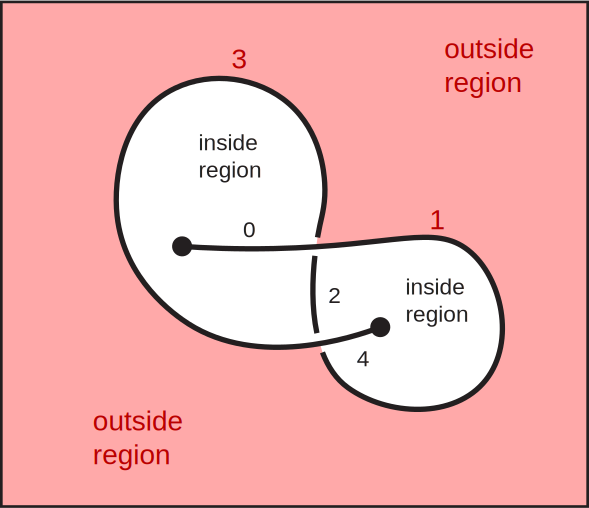
\includegraphics[scale=.35]{labeled_bifoil.pdf}
\caption{Labeled planar knotoid diagram corresponding to the PD code \lstinline{PD[X[2,r[1],r[3],0],X[r[1],4,2,r[3]]}.}\label{fig:labbif}
\end{figure}


Example of PD code for a knotoid diagram on the sphere (Figure~\ref{fig:labexamples} left):
\begin{lstlisting}
PD[
X[0,3,1,4],
X[4,1,5,2],
X[2,5,3,6]
];
\end{lstlisting}
It can also be written one line
\begin{lstlisting}
PD[X[0,3,1,4],X[4,1,5,2],X[2,5,3,6]];
\end{lstlisting}
Example of PD code for a knotoid diagram on the plane  (Figure~\ref{fig:labexamples} right):
\begin{lstlisting}
PD[
X[0,5,r[1],r[6]],
X[r[4],r[1],5,2],
X[7,2,8,3],
X[3,r[6],r[4],7]
];
\end{lstlisting}
and in one line
\begin{lstlisting}
PD[X[0,5,r[1],r[6]],X[r[4],r[1],5,2],X[7,2,8,3],X[3,r[6],r[4],7]];
\end{lstlisting}
Example of PD code for a knot diagram:
\begin{lstlisting}
PD[
X[0,3,1,4],
X[4,1,5,2],
X[2,5,3,0]
];
\end{lstlisting}
and in one line
\begin{lstlisting}
PD[X[0,3,1,4],X[4,1,5,2],X[2,5,3,0]];
\end{lstlisting}
\begin{figure}[t]
\centering
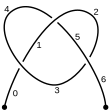
\includegraphics[scale=.35]{labeled_ex1.pdf}
\hspace*{2cm}
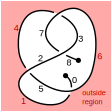
\includegraphics[scale=.35]{labeled_ex2.pdf}
\caption{Left: Labeled knotoid diagram corresponding to the PD code \lstinline{PD[X[0,3,1,4],X[4,1,5,2],X[2,5,3,6]]}. Right: Labeled knotoid diagram on the plane corresponding to the PD code \lstinline{PD[X[0,5,r[1],r[6]],X[r[4],r[1],5,2],X[7,2,8,3],X[3,r[6],r[4],7]]}.}\label{fig:labexamples}
\end{figure}

{\it Knoto-ID} also accept files with multiple diagrams. An example with two knotoid diagrams on the sphere:
\begin{lstlisting}
PD[X[3,1,4,0],X[1,5,2,4],X[5,3,6,2]];
PD[X[0,3,1,4],X[4,1,5,2],X[2,5,3,6]];
\end{lstlisting}
or simply concatenated in one line
\begin{lstlisting}
PD[X[3,1,4,0],X[1,5,2,4],X[5,3,6,2]];PD[X[0,3,1,4],X[4,1,5,2],X[2,5,3,6]];
\end{lstlisting}

The semicolons are not necessary and the following is also a valid list of diagrams
\begin{lstlisting}
PD[X[3,1,4,0],X[1,5,2,4],X[5,3,6,2]]PD[X[0,3,1,4],X[4,1,5,2],X[2,5,3,6]]
\end{lstlisting}

Finally, diagrams without crossings are allowed (Figure~\ref{fig:labempty}):
\begin{lstlisting}
PD[]
\end{lstlisting}

\begin{figure}[t]
\centering
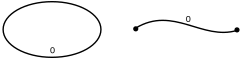
\includegraphics[scale=.35]{labeled_empty.pdf}
\caption{Left: Labeled knot diagram corresponding to the empty PD code \lstinline{PD[]}. Right: Labeled knotoid diagram corresponding to the empty PD code \lstinline{PD[]}.}\label{fig:labempty}
\end{figure}

\subsubsection{\label{sec:format:gauss}Knot(oid) diagrams (Extended Gauss code)}
Input and output format used to encode knot or knotoid diagrams based on the  extended Gauss codes\cite{gabrov,guka}. Extended gauss codes allows to encode knots and knotoid diagrams on the sphere and have the following form:
\[
\mbox{Gauss code} = \underbrace{\mbox{Crossings}}_{\mbox{first part}} \ \underbrace{\mbox{Signs}}_{\mbox{second part}}
\]

The {\bf first part} is a sequence of the crossings  of the diagram that is obtained by travelling around it, starting from one end and proceeding to the other, and labeling the crossings as we meet them (using strictly increasing non-negative integers). If we meet an undercrossing we note the crossing with a ``-'' sign, while if we meet an overcrossing we note it with a ``+'' sign. Note that each crossing is met twice in this trip and so each crossing will appear with both signs in the sequence. Therefore the length of this sequence is $2n$, where $n$ is the number of crossings. The case of knots is similar. The only difference is that we start the trip around the diagram from any arbitrary point. Note that different choices of starting points may yield different codes however, all codes will represent the same diagram. \\

The {\bf second part} is a sequence of the signs of each of the crossings of the diagram (Figure~\ref{crossings_v2}). Without it, the Gauss code represents a diagram up to its mirror image. The length of this sequence is $n$.\\

\begin{figure}[t]
\centering
\subfloat[]{
 \raisebox{-.1cm}{
\begin{tikzpicture}[scale=.5]
\draw [line width=0.8mm]  (-1,-1)-- (-0.22,-0.22);
\draw  [line width=0.8mm](-1,1)--(0,0);
\draw  [line width=0.8mm] (0.22,0.22) -- (1,1)[->];
\draw [line width=0.8mm]   (0,0) -- +(1,-1)[->];
\end{tikzpicture}}}   \hspace{3cm}
\subfloat[]{ \raisebox{-.1cm}{
\begin{tikzpicture}[scale=.5]
\draw  [line width=0.8mm] (-1,-1)-- (0,0) ;
\draw [line width=0.8mm] (-1,1)--(-0.22,0.22);
\draw [line width=0.8mm] (0,0) -- (1,1)[->];
\draw [line width=0.8mm]   (0.22,-0.22) -- +(.8,-.8)[->];
\end{tikzpicture}}}
\caption{A positive crossing with sign +1 (a) and a negative crossing with sign -1 (b).}\label{crossings_v2}
\end{figure}

For example, the knotoid diagram in Figure~\ref{fig:gc_example1} (left) corresponds to the following extended Gauss code:
\begin{lstlisting}
  -1 2 -3 1 -2 3 ---
\end{lstlisting}
\begin{figure}[t]
\centering
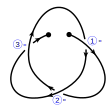
\includegraphics[width=0.25\textwidth]{gc_example2.pdf}\hspace{1cm}
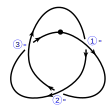
\includegraphics[width=0.25\textwidth]{gc_example3.pdf}
\caption{A knotoid diagram on the sphere and a knot diagram corresponding to the extended Gauss code \lstinline{-1 2 -3 1 -2 3 ---}. Crossing labels and signs are shown in blue.}\label{fig:gc_example1}
\end{figure}
Another example is the knotoid diagram shown in Figure~\ref{fig:gc_example4}, which corresponds to the following extended Gauss code:
\begin{lstlisting}
  1 -2 3 -1 -4 -5 2 -3 5 4 +++-+
\end{lstlisting}
\begin{figure}[t]
\centering
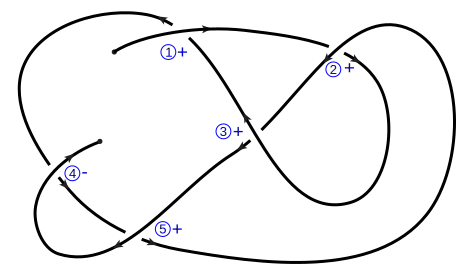
\includegraphics[width=0.6\textwidth]{gc_example5.pdf}
\caption{A labeled knotoid diagram corresponding to the extended Gauss code \lstinline{1 -2 3 -1 -4 -5 2 -3 5 4 +++-+}. Crossing labels and signs are shown in blue.}\label{fig:gc_example4}
\end{figure}

Except for pure knotoids, it is not possible to know whether a diagram is open or closed based only on its extended Gauss code. For example, both the knotoid diagram and the knot diagram in Figure~\ref{fig:gc_example1} correspond to the same extended Gauss code. Therefore, when loading a diagram from a Gauss code, one has to additionally specify whether it is open or closed using option \lstinline{--closure-method=open} (open diagram) or \lstinline{--closure-method=direct} or \lstinline{rays} (closed diagram). 


This form of extended Gauss codes cannot be used for planar diagrams as the information on which arcs touch the outside region is missing. For example, both knotoids diagrams in Figure~\ref{fig:gc_example2} correspond to the same extended Gauss code \lstinline{-1 2 -3 1 -2 3 ---}.
\begin{figure}[t]
\centering
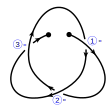
\includegraphics[width=0.25\textwidth]{gc_example2.pdf}\hspace{1cm}
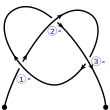
\includegraphics[width=0.25\textwidth]{gc_example1.pdf}
\caption{Two knotoid diagrams corresponding to the extended Gauss code \lstinline{-1 2 -3 1 -2 3 ---}. Crossing labels and signs are shown in blue.}\label{fig:gc_example2}
\end{figure}

To overcome this limitation, Knoto-ID accepts a modified version of the extended Gauss code, which allows the encoding of planar and spherical knotoid diagrams as well as knot diagrams. Such a code has the following form:
\[
\mbox{Gauss code} = \underbrace{\mbox{Crossings}}_{\mbox{first part}} \ \underbrace{\mbox{Signs}}_{\mbox{second part}} \ \underbrace{\mbox{Outside arcs}}_{\mbox{third part}}
\]

The {\bf first part} and {\bf second part} encode information on the crossings, as described previously.\\

The {\bf third part} allows the proper encoding of a planar knotoid diagram. It consists in a list of arc labels corresponding to the arcs of the diagram that are adjacent to the outside region of the diagram. This part has no fixed length. Note that arcs must be labeled with integer numbers, starting from 0 for the first arc and increasing by steps of 1 for each subsequent arc that is met when traveling along the curve.\\


For example, the knotoid diagram in Figure~\ref{fig:gc_example3} corresponds to the following extended Gauss code:
\begin{lstlisting}
  1 -2 3 -1 -4 -5 2 -3 5 4 +++-+ 0 3 4 5 8 10
\end{lstlisting}
\begin{figure}[t]
\centering
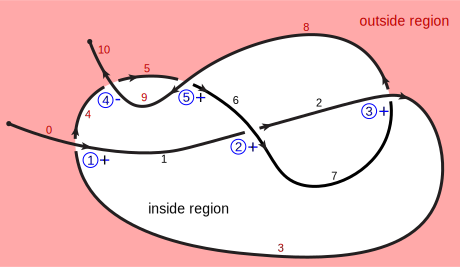
\includegraphics[width=0.6\textwidth]{gc_example4.pdf}
\caption{Labeled knotoid diagram corresponding to the extended Gauss code \lstinline{1 -2 3 -1 -4 -5 2 -3 5 4 +++-+ 0 3 4 5 8 10}. Crossing labels and signs are shown in blue. Arc labels are shown in red for arcs adjacent to the outside region and black for internal arcs.}\label{fig:gc_example3}
\end{figure}


Notes:
\begin{itemize}
\item For diagrams without crossings (Figure~\ref{fig:labempty}), the special keyword \lstinline{empty_diagram} is used.
\item When specifying whether a diagram is open or closed (with \lstinline{--closure-method}) care must be taken to avoid unrealisable diagrams. Two typical sources of mismatch between diagram topology and the choice of closure are:
\begin{itemize}
\item Closing a pure knotoid diagram. For example, the knotoid diagram in Figure~\ref{fig:labbif} with extended Gauss code \lstinline{1 -2 -1 2 ++ 1 3} cannot be closed without creating additional crossings. Note that {\it Knoto-ID} may read such a Gauss code without detecting that it does not correspond to realisable knot(oid) diagram. However this will lead to unpredictable output.
\item  Closing a planar knotoid diagram with its last endpoint in the outside region. For example, in the knotoid diagram shown in Figure~\ref{fig:gc_example3}, the last endpoint is outside and arc 10 appears in the extended Gauss code \lstinline{1 -2 3 -1 -4 -5 2 -3 5 4 +++-+ 0 3 4 5 8 10}. If we ask {\it Knoto-ID} to consider this diagram closed, it will complain that arc 10 does not exist ( arc 10 is merged arc 0 when closing the diagram).
\end{itemize}
\item While the labeling of arcs is very strict (starting from 0, increasing by steps of 1 when following the curve), labeling of nodes is more flexible. The only requirements are that node labels are non negative integer, and that the label increase when following the curve and meeting a crossing for the time.
All the following Gauss code correspond to the diagram shown in Figure~\ref{fig:gc_example3} (although with different labeling of the crossings):
\begin{lstlisting}
  1 -2 3 -1 -4 -5 2 -3 5 4 +++-+ 0 3 4 5 8 10
\end{lstlisting}
\begin{lstlisting}
  0 -1 2 -0 -3 -4 1 -2 4 3 +++-+ 0 3 4 5 8 10
\end{lstlisting}
but also
\begin{lstlisting}
  0 -5 7 -0 -10 -12 5 -7 12 10 +++-+ 0 3 4 5 8 10
\end{lstlisting}
Note that {\it Knoto-ID} relabels the crossings when loading a diagram from an extended Gauss code. Therefore the crossing labels in output may not correspond to the labels used in input. 
\item When reading an extended Gauss code, {\it Knoto-ID} replaces the following characters by blank space: \lstinline{[}, \lstinline{]}, \lstinline{(}, \lstinline{)}, \lstinlineT{\{}, \lstinlineT{\}}, \lstinline{,} and \lstinline{;}. As a consequence, the input format is quite flexible and all the following expressions are valid extended Gauss codes representing the knotoid diagram in  Figure~\ref{fig:gc_example2}:
\begin{lstlisting}
  {1,-2,3,-1,-4,-5,2,-3,5,4} {+++-+} {0,3,4,5,8,10}
\end{lstlisting}
\begin{lstlisting}
  (1 -2 3 -1 -4 -5 2 -3 5 4) (+ + + - +) (0 3 4 5 8 10)
\end{lstlisting}
\begin{lstlisting}
  1,-2,3,-1,-4,-5,2,-3,5,4,+,+,+,-,+,0,3,4,5,8,10
\end{lstlisting}
\end{itemize}

{\it Knoto-ID} also accept files with multiple diagrams, with one extended Gauss code per line. An example with two diagrams:
\begin{lstlisting}
1 -2 3 -1 2 -3 +++  
-1 2 -3 1 -2 3 ---
\end{lstlisting}



\subsubsection{\label{sec:format:multiprojection:jones}Distribution of polynomials}
Output format used to characterize the distribution of polynomials obtained with multiple projections. This is a tab separated format with 2 mandatory columns (frequency and polynomial) and 1 optional column (knot or knotoid type).
The first row is a header (starting with \#) specifying the label of each column.
In each subsequent row, the entry in column frequency is the fraction of all projections that gave the corresponding polynomial, followed optionally by the knot or knotoid type corresponding to the polynomial. Note that if weights were associated with the projections\footnote{see section ``\ref{sec:format:projections} \nameref{sec:format:projections}'' for more details.}, the column frequency contains the weighted fraction.

Example, without knot type:
\begin{lstlisting}
#frequency  polynomial
0.9         - A^(-16) + A^(-12) + A^(-4)
0.1         + 1
\end{lstlisting}
Example, with knot type:
\begin{lstlisting}
#frequency  knot_type  polynomial
0.7         3_1R       - A^(-16) + A^(-12) + A^(-4)
0.3         0_1        + 1
\end{lstlisting}



\subsubsection{\label{sec:format:multiprojection:diagrams}List of projections with polynomials and knot(oid) diagrams}
Tab separated output format with 5 columns (x, y, z coordinates of the projection direction, polynomial invariant and knot(oid) diagram) and  1 optional column (knot or knotoid type).
The first row is a header (starting with \#) specifying the label of each column.
With the optional column for the knot(oid) type, each subsequent row corresponds to a single projection direction (columns 1 to 3) together with the knot(oid) type (column 4), the polynomial (column 5) and PD code\footnote{see section ``\ref{sec:format:pd} \nameref{sec:format:pd}'' for more information on the file format.} or extended Gauss code\footnote{see section ``\ref{sec:format:gauss} \nameref{sec:format:gauss}'' for more information on the file format.} for the knot(oid) diagram (column 6) obtained from this projection.

Without the optional column for the knot(oid) type, the polynomial is given in column 4 and the PD code or extended Gauss code for the knot(oid) diagram is in column 5.


Example (without knot(oid) names):
\begin{lstlistingverysmall}
#projection.x  projection.y  projection.z  polynomial                    PD_code
0.483595       -0.85801      0.173072      - A^(-16) + A^(-12) + A^(-4)  PD[X[3,1,4,0],X[1,5,2,4],X[5,3,6,2]];
0.521928       -0.578265     0.627058      - A^(-16) + A^(-12) + A^(-4)  PD[X[3,1,4,0],X[1,5,2,4],X[5,3,6,2]];
0.898137       0.241849      0.367231      - A^(-16) + A^(-12) + A^(-4)  PD[X[7,0,8,1],X[4,2,5,1],X[2,6,3,5],X[6,4,7,3]];
-0.624015      0.596182      0.505146      - A^(-10) + A^(-6) + A^(-4)   PD[X[0,3,1,2],X[3,2,4,1]];
0.134038       -0.988518     -0.0697575    - A^(-16) + A^(-12) + A^(-4)  PD[X[5,1,6,0],X[1,5,2,4],X[2,8,3,7],X[6,4,7,3]];
\end{lstlistingverysmall}
Example (with knot(oid) names):
\begin{lstlistingverysmall}
#projection.x projection.y projection.z knotoid_type polynomial                   PD_code
0.483595      -0.85801     0.173072     k3.1o       - A^(-16) + A^(-12) + A^(-4)  PD[X[3,1,4,0],X[1,5,2,4],X[5,3,6,2]];
0.521928      -0.578265    0.627058     k3.1o       - A^(-16) + A^(-12) + A^(-4)  PD[X[3,1,4,0],X[1,5,2,4],X[5,3,6,2]];
0.898137      0.241849     0.367231     k3.1o       - A^(-16) + A^(-12) + A^(-4)  PD[X[7,0,8,1],X[4,2,5,1],X[2,6,3,5],X[6,4,7,3]];
-0.624015     0.596182     0.505146     k2.1        - A^(-10) + A^(-6) + A^(-4)   PD[X[0,3,1,2],X[3,2,4,1]];
0.134038      -0.988518    -0.0697575   k3.1o       - A^(-16) + A^(-12) + A^(-4)  PD[X[5,1,6,0],X[1,5,2,4],X[2,8,3,7],X[6,4,7,3]];
\end{lstlistingverysmall}
Example with extended Gauss code instead of PD code:
\begin{lstlistingverysmall}
#projection.x projection.y projection.z knotoid_type polynomial                    gauss_code
0.483595      -0.85801     0.173072     k3.1o       - A^(-16) + A^(-12) + A^(-4)   1 -2 3 -1 2 -3 +++
0.521928      -0.578265    0.627058     k3.1o       - A^(-16) + A^(-12) + A^(-4)   1 -2 3 -1 2 -3 +++
0.898137      0.241849     0.367231     k3.1o       - A^(-16) + A^(-12) + A^(-4)   1 2 -3 4 -2 3 -4 -1 -+++
-0.624015     0.596182     0.505146     k2.1        - A^(-10) + A^(-6) + A^(-4)    -1 2 1 -2 ++
0.134038      -0.988518    -0.0697575   k3.1o       - A^(-16) + A^(-12) + A^(-4)   1 -2 -3 4 2 -1 -4 3 ++++
\end{lstlistingverysmall}


\subsubsection{\label{sec:format:projections}List of projections}
Tab (or space) separated input format with 3 mandatory columns (x, y, z coordinates of the projection direction) and 1 optional column (weight)
The first row can optionally contain a header starting with \#.
Each subsequent row defines one projection direction with an optional weight (set to 1 if missing). The weight is used when evaluating the distribution of polynomials (the fraction of projections is replaced by a weighted fraction of projections)

Example:
\begin{lstlisting}
#projection.x  projection.y  projection.z  weight
0              0             1             1
0              1             0             1
1              0             0             1
0              0             -1            1
0              -1            0             1
-1             0             0             1
\end{lstlisting}



\subsubsection{\label{sec:format:namesdb}List of knot(oid) names}
Tab separated input format with 2 columns used to specify the correspondence between polynomials and knot(oid) names. Each row contains a knot or knotoid name in the first column and the corresponding polynomial in the second column.
While any string are accepted as a knot or knotoid name (as long as it does not contain a tab character), the polynomials must conform to the ``Polynomial'' format described in  section ``\ref{sec:format:polynomials} \nameref{sec:format:polynomials}''.

Two rows may contain the same polynomial with a different knot(oid) names. All knot(oid) names corresponding to the same polynomial will be concatenated  with a \lstinline{|} separator. For example, knots 6\_2R and 12n\_0025L have the same classical Jones polynomial $-1 + A^{-20} - 2 A^{-16} + 2 A^{-12} - 2 A^{-8} + 2 A^{-4} + A^4$ and the  corresponding knot name will be \lstinline{6_2R|12n_0025L}.


Example of list of knot names:
\begin{lstlisting}
0_1     1
3_1R    -A^(-16) + A^(-12) + A^(-4)
3_1L    A^4 + A^12 - A^16
4_1     1 + A^(-8) - A^(-4) - A^4 + A^8
5_1R    -A^(-28) + A^(-24) - A^(-20) + A^(-16) + A^(-8)
5_1L    A^8 + A^16 - A^20 + A^24 - A^28
5_2R    -A^(-24) + A^(-20) - A^(-16) + 2*A^(-12) - A^(-8) + A^(-4)
5_2L    A^4 - A^8 + 2*A^12 - A^16 + A^20 - A^24
6_1R    2 + A^(-16) - A^(-12) + A^(-8) - 2*A^(-4) - A^4 + A^8
6_1L    2 + A^(-8) - A^(-4) - 2*A^4 + A^8 - A^12 + A^16
6_2R    -1 + A^(-20) - 2*A^(-16) + 2*A^(-12) - 2*A^(-8) + 2*A^(-4) + A^4
6_2L    -1 + A^(-4) + 2*A^4 - 2*A^8 + 2*A^12 - 2*A^16 + A^20
6_3     3 - A^(-12) + 2*A^(-8) - 2*A^(-4) - 2*A^4 + 2*A^8 - A^12
\end{lstlisting}



\subsubsection{\label{sec:format:polynomials}Polynomials}
Polynomials are used both as input\footnote{section ``\ref{sec:format:namesdb} \nameref{sec:format:namesdb}''} and output\footnote{sections ``\ref{sec:format:multiprojection:jones} \nameref{sec:format:multiprojection:jones}'', ``\ref{sec:format:multiprojection:diagrams} \nameref{sec:format:multiprojection:diagrams}''.}.

Classical Jones polynomial and Jones polynomial for knotoids are univariate Laurent polynomials in variable $A$ with integer coefficients.
Turaev loop bracket polynomial is a bivariate Laurent polynomial in variables $A$ and $v$ with integer coefficients. See section ``\ref{sec:theory:jones} \nameref{sec:theory:jones}'' for more details.

For the file format, we consider the more general case of bivariate Laurent polynomial with integer coefficients. It should be written as a sum of monomials:
\[\sum_{n,m} C_{n,m}A^nv^m\text{ with }n,m,C_{n,m}\in\mathbb Z \]
Each monomial must be written using operators \lstinline{*} for multiplication and  \lstinline{^} for exponentiation:
\begin{lstlisting}
2*A^2*v^8
\end{lstlisting}

For clarity, exponents can be written between brackets
\begin{lstlisting}
2*A^(-4)*v^(2)
\end{lstlisting}
but it is not mandatory:
\begin{lstlisting}
2*A^-4*v^2
\end{lstlisting}
will also be interpreted as $2A^{-4}v^{2}$.

Terms with exponent 0 can be replaced by 1. For example \lstinline{2*A^(-4)*v^(0)} can be replaced by \lstinline{2*A^(-4)} and  \lstinline{2*A^(0)*v^(0)} can be replaced by \lstinline{2}.

Exponent 1 can be removed. For example \lstinline{2*v^(1)} can be replaced by \lstinline{2*v}.

Coefficient 1 can be removed for terms with non-zero exponent. For example  \lstinline{1*A^(-4)*v^(8)} can be replaced by \lstinline{A^(-4)*v^(8)} and   \lstinline{1*A^(-4)} can be replaced by \lstinline{A^(-4)}.

Finally, monomials must be combined with addition and subtraction operators (\lstinline{+} and \lstinline{-}):
\begin{lstlisting}
1 + A^(-8) - A^(-4) - A^4 + A^8
\end{lstlisting}
The first monomial can be prefixed by a unary sign operator
\begin{lstlisting}
-A^(-16) + A^(-12) + A^(-4)
\end{lstlisting}
Note that the combination of the binary addition or substraction operators with unary sign operator is not allowed: \lstinline{ + -A^2}, \lstinline{A^2 + -v^4} or \lstinline{A^2 - -v^4} will all generate an error.

Space character is allowed and can be used to improve readability but it is ignored.

Examples of valid polynomials:
\begin{lstlisting}
1
\end{lstlisting}
\begin{lstlisting}
-A^(-4) - 4*A^(-2)*v
\end{lstlisting}
\begin{lstlisting}
-A^2*v - A^4
\end{lstlisting}
\begin{lstlisting}
-A^-10 + A^-6 + A^-4
\end{lstlisting}
\begin{lstlisting}
1 + A^(-2) + v + A^(2)
\end{lstlisting}
\begin{lstlisting}
+A^(-8) + A^(-6)*v^(-4) - A^(-2)*v
\end{lstlisting}



  
\subsubsection{\label{sec:format:listsubchains}List of subchains}
Output format used by \lstinline{knotted_core} program to output the dominant knot(oid) of subchains of the input curve.
This is a tab separated format with 5 mandatory columns (first and last indices of the subchain, length of the subchain, frequency and polynomial)  and 1 optional column (Knot or knotoid type).
The first row is a header (starting with \#) specifying the label of each column.
Each subsequent row corresponds to one subchain, defined by its first and last indices (using zero-based indexing) as well as the length of the subchain (number of points). In addition, the corresponding dominant polynomial is given, together with its frequency (fraction of all projections that have the corresponding polynomial). Optionally, the Knot or knotoid type corresponding to the polynomial can also be given.

Each subchain is defined by a first index  and a length. Although not necessary to define the subchain, its last index is also given for completeness. Given a first index $i_1$, a length $l$ and a last index $i_2:=i_1+l-1{\rm\ mod\ } N$, the subchain is defined by the ordered set of points of the input curve with indices:
\[\{i_1{\rm\ mod\ } N,(i_1+1){\rm\ mod\ } N,\cdots,(i_1+l-1){\rm\ mod\ } N\}\]
where N is the number of points in the input curve (See Figures~\ref{fig:subchains:open} and \ref{fig:subchains:closed}).  
\begin{figure}[t]
\centering
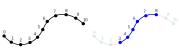
\includegraphics[width=0.6\textwidth]{subchains_open.pdf}
\caption{Left: open input curve with $N=11$ points. Right: a subchain with first index $i_1=3$, length $l=6$ and last index $i_2=8$ (blue).}\label{fig:subchains:open}
\end{figure}
\begin{figure}[t]
\centering
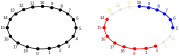
\includegraphics[width=0.6\textwidth]{subchains_closed.pdf}
\caption{left: closed input curve with $N=19$ points. Right: a subchain with first index $i_1=5$, length $l=6$ and last index $i_2=10$ (blue), and a  subchain with first index $i_1=14$, length $l=8$ and last index $i_2=2$ (red).}\label{fig:subchains:closed}
\end{figure}

Note: by definition, $l>N$ corresponds to the full input curve closed with direct closure.


Example for an open chain, without knot(oid) type:
\begin{lstlisting}
#index_first  index_last  length  frequency  polynomial
11            51          41      0.7        - A^(-10) + A^(-6) + A^(-4)
12            52          41      0.75       - A^(-16) + A^(-12) + A^(-4)
13            52          40      0.85       - A^(-16) + A^(-12) + A^(-4)
14            52          39      0.75       - A^(-16) + A^(-12) + A^(-4)
\end{lstlisting}

Example for a closed chain (with $N=111$ points), with knot type:
\begin{lstlisting}
#index_first  index_last  length  frequency  knot_type  polynomial
22            110         89      0.8        3_1R       - A^(-16) + A^(-12) + A^(-4)
22            0           90      0.5        3_1R       - A^(-16) + A^(-12) + A^(-4)
23            1           90      0.6        3_1R       - A^(-16) + A^(-12) + A^(-4)
22            79          58      0.8        3_1R       - A^(-16) + A^(-12) + A^(-4)
23            23          112     1          3_1R       - A^(-16) + A^(-12) + A^(-4)
\end{lstlisting}
Note that the length of last subchain is bigger than the number of input points, therefore the last subchain corresponds to the full input curve (with direct closure).

\subsubsection{\label{sec:format:xyzdiagrams}xyz format for knot(oid) diagrams} 
Tab (or space) separated output format with 4 columns corresponding to x, y, z coordinates and a label.
The first row is a header (starting with \#) specifying the label of each column.
Each subsequent row corresponds to a point of the curve. Consecutive points (rows) will be connected by a straight line. Note that consecutive lines may have the same x, y, z coordinates.
This format is used by \lstinline{convert_diagram} to output planar represenations of knot(oid) diagrams in the xy plane. The z coordinate ranges from -1 to +1 and is used to specify which arc is above ($z>0$) or below ($z<0$) at each crossing.

The following example corresponds to a knot diagram with two arcs and one crossing:
\begin{lstlisting}
#x y z label
0.728017   0.387851      0.698611   Arc_0
0.960894   0.511916      0.358889   Arc_0
1.02482    0.255915      0          Arc_0
1.02482    0.255915      0          Arc_0
1.08874    -8.68623e-05  -0.358889  Arc_0
0.824876   -6.58107e-05  -0.698611  Arc_0
0.824876   -6.58107e-05  -0.698611  Crossing_0
0          0             -1         Crossing_0
-0.824876  3.29053e-05   -0.698611  Crossing_0
-0.824876  3.29053e-05   -0.698611  Arc_1
-1.08874   4.34311e-05   -0.358889  Arc_1
-1.02481   -0.255956     0          Arc_1
-1.02481   -0.255956     0          Arc_1
-0.960873  -0.511954     0.358889   Arc_1
-0.728001  -0.38788      0.698611   Arc_1
-0.728001  -0.38788      0.698611   Crossing_0
0          0             1          Crossing_0
0.728017   0.387851      0.698611   Crossing_0
\end{lstlisting}

\clearpage

% Copyright (C) 2017 by SIB Swiss Institute of Bioinformatics, Julien Dorier and Dimos Goundaroulis.
% 
% This file is part of project Knoto-ID.
% 
% Knoto-ID is free software: you can redistribute it and/or modify
% it under the terms of the GNU General Public License as published by
% the Free Software Foundation, either version 2 of the License, or
% (at your option) any later version.
% 
% Knoto-ID is distributed in the hope that it will be useful,
% but WITHOUT ANY WARRANTY; without even the implied warranty of
% MERCHANTABILITY or FITNESS FOR A PARTICULAR PURPOSE.  See the
% GNU General Public License for more details.
% 
% You should have received a copy of the GNU General Public License
% along with Knoto-ID.  If not, see <http://www.gnu.org/licenses/>.

\section{\label{sec:theory}Theory}
\subsection{\label{sec:theory:knots}Knots}
A knot is a smooth embedding of a circle into $\mathbb{R}^3$, considered up to continuous deformations. To be more precise, a knot is a closed curve in 3-dimensional Euclidean space that does not intersect itself anywhere and can be continuously deformed as if it was made of rubber\cite{Adams}.  Knots are usually studied through their diagrams, which are abstract and schematized pictures of a knot composed of curves in the plane that cross transversely in 4-fold vertices. Each vertex is equipped with extra structure in the form of a deleted segment that indicates the under crossing line and they are called {\it crossings} of the knot. With this information, one is always able to reconstruct the knot in 3-space (see Fig.~\ref{fig:knotdiag}).
\begin{figure}[h]
\centering
\subfloat[]{

\begin{tikzpicture}[scale=.8]
\draw [line width=0.8mm]  (-1,-1)-- (-0.22,-0.22);
\draw  [line width=0.8mm ](-1,1)--(0,0);
\draw  [line width=0.8mm] (0.22,0.22) -- (1,1);
\draw [line width=0.8mm]   (0,0) -- +(1,-1);
\end{tikzpicture}}\hspace{3cm}
\subfloat[]{\includegraphics[scale=.13]{figure1}}
\caption{A crossing (a) and a knot diagram (b).}\label{fig:knotdiag}
\end{figure}


Two knots are equivalent, that is they can be deformed to one another, if and only if their diagrams can be transformed to one another by a finite sequence of three elementary diagram moves called the Reidemeister moves (see Fig.~\ref{fig:rmoves}) along with planar isotopy. Planar isotopy is a motion of the diagram in the plane that preserves the underlying structure. These tools work efficiently well for distinguishing knots with small number of crossings, however, for knots with higher number of crossings (see Fig.~\ref{fig:unknot}) more sophisticated tools are required.
\begin{figure}[h]
\centering

\includegraphics[scale=.3]{figure2}
\caption{Louis Kauffman's unknot. This rather complicated knot is actually equivalent to the trivial knot.}\label{fig:unknot}
\end{figure}

 Such tools are the so-called knot invariants and are functions defined on the set of all knots and links that assign the same value to equivalent knots or links. In this work we focus on the classical Jones polynomial for knots \cite{jones} and the various extensions of the Kauffman bracket polynomial \cite{kauffman1988} to the case of knotoids\cite{turaev,guka,gound2,goundaroulis2019}.

\begin{figure}[h]
\centering
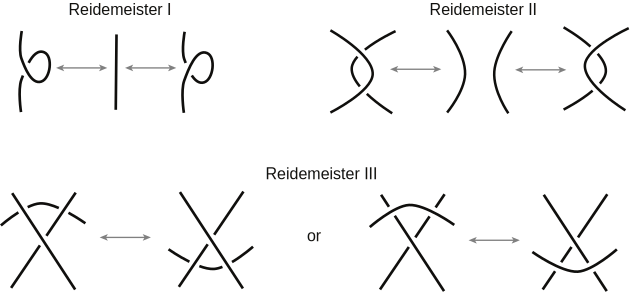
\includegraphics[scale=.93]{figure3}
\caption{The three Reidemeister moves.}\label{fig:rmoves}
\end{figure}


\subsection{\label{sec:theory:knotoids}Knotoids}
Consider that we started drawing a knot diagram and at some point in this process we decided to leave the diagram open, i.e. not to connect the end points. The question now is if this allows the definition of open knot diagrams. It is not difficult to see that if we apply planar isotopy and the Reidemeister moves as described above to such a diagram, eventually we will always manage to unknot it. However, if we require the Reidemeister moves to be applied only at local neighbourhoods of the diagram that don't involve the endpoints we are getting closer to the notion of open knotting. Additionally, if we forbid the endpoints to slide over or under the rest of the diagram (see Fig.~\ref{fig:forbidden}), then we have achieved our goal. 

\begin{figure}[h]
\centering
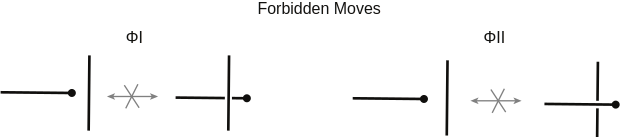
\includegraphics[scale=1]{figure4}
\caption{The two forbidden moves.}\label{fig:forbidden}
\end{figure}

What we have just described is a {\it knotoid diagram}. Knotoid diagrams generalize the notion of a 1-1 tangle (or a long knot) since they allow the endpoints to be in different regions of the diagram, and thus they provide a rigorous definition for open knots. Their equivalence classes under the forbidden moves as well as the Reidemeister moves away from the endpoints  are called {\it knotoids} (see Fig.~\ref{fig:knotoid}). Knotoids were first introduced by V. Turaev in\cite{turaev} and have been studied further by L. Kauffman and N. G\"ug\"umc\"u in\cite{guka}.  Formally, a knotoid is defined as the generic  immersion  of  the  closed unit interval  in  the  interior  of the surface whose  only  singularities are  transversal  double  points  endowed  with  over/undercrossing  data. In analogy to the case of knots, the double points of the knotoid diagram are also called crossings.   The  images  of  0 and  1  under  this  immersion  are  called  the {\it tail} and  the {\it head} of the knotoid diagram,  respectively, they are  distinct  from  each other  and from  the  double  points.  Every knotoid diagram comes with an orientation the goes from the tail to the head\cite{turaev}.  Knotoids that have both ends in the same region of the diagram are called {\it knot-type} knotoids while knotoids that have their end points in different regions of the diagram are called {\it proper} knotoids.

\begin{figure}[h]
\centering
\includegraphics[scale=.35]{figure5}
\caption{Examples of knotoids. The diagram (c) corresponds to a knot-type knotoid while (a), (b) and (d) to proper knotoids.}\label{fig:knotoid}
\end{figure}

Knotoids are defined on an oriented surface but they are usually studied on the surface of the 2-sphere $S^2$ but their definition can also be extended to the plane $\mathbb{R}^2$. We shall call this class of knotoids {\it planar}. There are pairs non-isotopic planar knotoids that become isotopic once we consider them as knotoids on $S^2$. For example, in Figure~\ref{fig:knotoid}, diagrams (a) and (b) are not equivalent as planar knotoids but they become equivalent once they are considered in $S^2$. This is because on the sphere one has the freedom to move arcs using isotopy towards/over the poles and around the sphere in order to simplify the diagram, something that is not possible while working on the plane.


One can recover a knot diagram from a knotoid diagram $k$ by embedding an arc $\alpha$ that passes everywhere under $k$ and connect the endpoints of $k$ to $\alpha$. The arc is called a {\it shortcut} for $k$ and the way of closure is called the {\it underpass} closure  (See Figure~\ref{fig:closure}). The shortcut is unique for every knotoid diagram, up to isotopy. In an analogous way one can define the {\it overpass closure}\cite{turaev, guka}. On the other hand, every knot may be presented by a knotoid diagram by cutting out an underpassing arc\cite{turaev}.


\begin{figure}[h]
\centering
\includegraphics[scale=.35]{figure6}
\caption{Knotoids to knots using the underpass closure. The embedded arc $\alpha$ is shown in red.}\label{fig:closure}
\end{figure}





\subsection{\label{sec:theory:knotoidsandcurves}Knotoids and curves in space}

Consider an embedded open curve in space. We would like to know if it is entangled or not. One may suggest to project the curve on a plane and study its projection as a knotoid diagram and they would be partially right. However, how can we be sure that by accidentally perturbing a bit the curve we don't mess with its topology? In order to avoid situations like this we first introduce two infinite lines that pass through the endpoints of the curve. In this way all manipulations of the curve in space with respect to these two lines preserve the topology of the curve\cite{guka}. Finally, the curve is projected on  an orientable surface (e.g. a sphere, a plane, etc.), and thus a knotoid diagram is obtained. 

Note now that different choices of projection planes will possibly lead to different knotoid diagrams. For this reason, in order to study the topology of an embedded open curve we work as follows. We assume that the curve lies inside a large enough sphere (a radius of twice the length of the curve will do fine for most of the cases). Each point of the sphere corresponds to a vector that points towards an orientable surface that lies outside of the sphere (see Figure~\ref{fig:project}). For each choice of the projection surface we introduce the infinite parallel lines and we take the projection of the curve together with the information of over/under crossing arc at each double point. The knotoid type is then evaluated using an invariant for knotoids. Thus, the entanglement of the embedded open curve is a probability distribution that we can approximate by sampling the sphere\cite{gound}.
\begin{figure}[h]
\centering
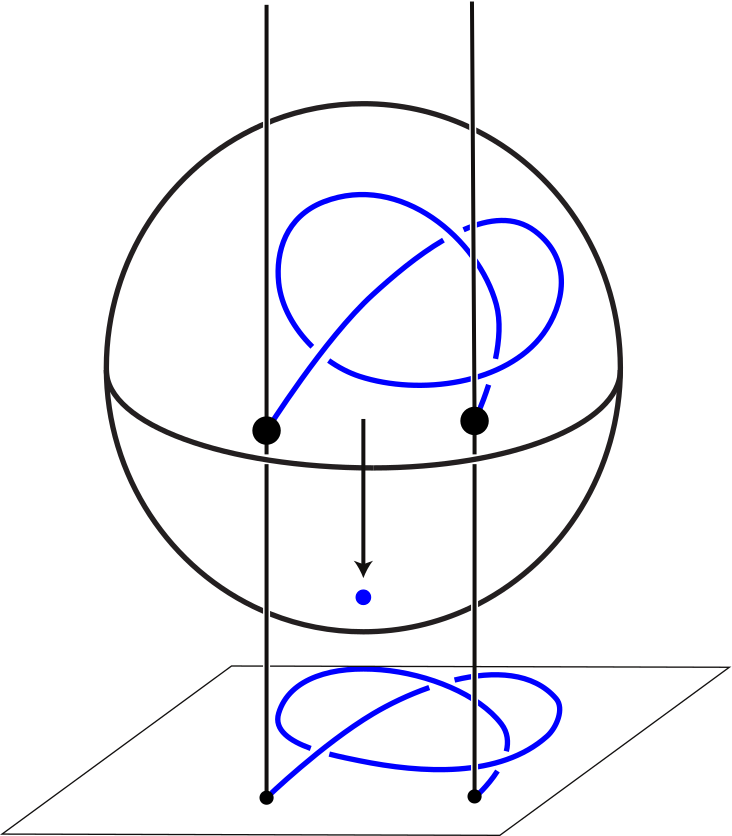
\includegraphics[scale=.3]{figure7}
\caption{ The curve is placed inside a large sphere. The blue dot indicates a vector that points towards an oriented surface of projection (plane or sphere). The two infinite parallel lines are introduced and the curve is projected on the chosen oriented surface.}\label{fig:project}
\end{figure}


The equivalent of the over/underpassing closure for the case of embedded open curves is most probably the uniform (or stochastic) closure technique\cite{mansfield1994, sulkowska2012, lua2006,millett2004, jamroz2014}.
Here the curve is placed again inside a large ball, only this time each point of the sphere corresponds to a closure direction. The closure is achieved by extending two parallel rays, each originating from one of the endpoints of the curve, towards that the chosen closure direction and they are connected outside of the sphere (see Figure~\ref{fig:closure}).
This method is, as hinted by its name, also probabilistic and so the knot-type of the core is a probability distribution of all knot-types obtained by closing over all possible directions that are defined by the points of the sphere.
There is however the option to close the open curve using an arc that directly connects the endpoints\cite{taylor2000,virnau2006} (direct closure method). This method is computationally faster but it may interfere with the topology of the chain by introducing or removing crossings. In contrast to the direct closure technique, the stochastic closure provides more detailed overview but it is computationally more demanding as one is required to sample a probability distribution in order to understand the topology of the studied object.
\begin{figure}[h]
\centering
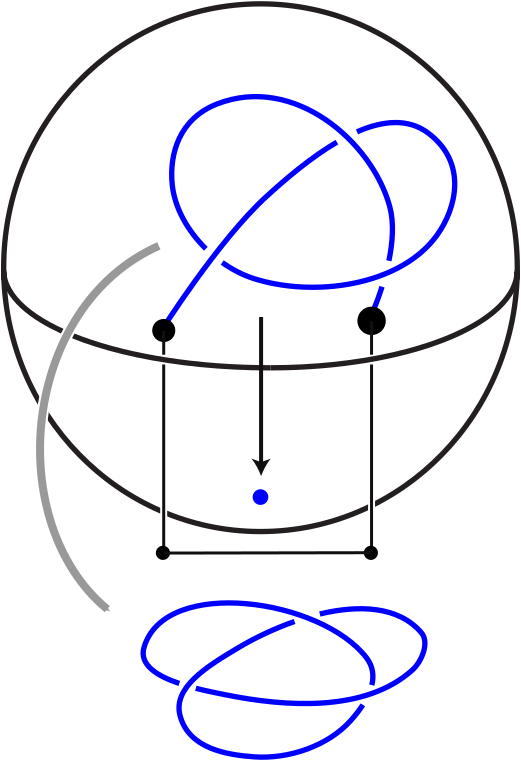
\includegraphics[scale=.3]{figure8}
\caption{The uniform (or stochastic) closure technique. Two parallel rays are extended towards the closure direction indicated by the blue point and they are connected outside of the sphere. The resulting knot may be evaluated using a knot invariant.}\label{fig:stochastic}
\end{figure}

\subsection{\label{sec:theory:jones}Computing polynomial invariants}
In this section we will present the Kauffman bracket\cite{kauffman1988} and how it gives rise to the classical Jones polynomial for knots\cite{jones}, the Jones polynomial for knotoids\cite{turaev,guka} and the Turaev loop bracket polynomial for planar knotoids\cite{turaev}. Moreover, we present how we can obtain the arrow polynomial \cite{dye2009,guka} from the oriented extension of the Kauffman bracket. Finally, we give the planar extension of the arrow polynomial, the loop arrow polynomial \cite{gound2, goundaroulis2019}

\subsubsection{\label{sec:theory:jones:classicaljones}Classical Jones polynomial for knots}
Consider  a knot $K$ and observe that a each crossing \raisebox{-.1cm}{
\begin{tikzpicture}[scale=.2]
\draw [line width=0.35mm]  (-1,-1)-- (-0.22,-0.22);
\draw  [line width=0.35mm ](-1,1)--(0,0);
\draw  [line width=0.35mm] (0.22,0.22) -- (1,1);
\draw [line width=0.35mm]   (0,0) -- +(1,-1);
\end{tikzpicture}} of $K$ can be smoothed in two different ways. The first way is to smooth it horizontally \raisebox{-.07cm}{
\begin{tikzpicture}[scale=.2]
\draw [line width=0.35mm] plot [smooth, tension=2] coordinates { (-1,.8) (0, 0.5) (1,.8)};
\draw [ line width=0.35mm] plot [smooth, tension=2] coordinates { (-1,-.8) (0, -0.5) (1,-.8)};
\end{tikzpicture}} and the second is to smooth it vertically  \raisebox{-.1cm}{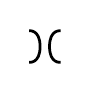
\begin{tikzpicture}[scale=.2]
 \draw [ line width=0.35mm] plot [smooth, tension=2] coordinates { (-1,-1) (-0.3, 0) (-1,1)};
 \draw [ line width=0.35mm] plot [smooth, tension=2] coordinates { (1,-1) (0.3, 0) (1,1)};
 \end{tikzpicture}}. If $K$ has $n$ crossings then  there are $2^n$ possible smoothings of $K$. With these in mind we define the Kauffman bracket as the 1-variable polynomial $\langle K \rangle \in \mathbb{Z}[A,A^{-1}]$ that satisfies the following axioms:


\begin{eqnarray}
&&\langle \raisebox{-.1cm}{
\begin{tikzpicture}[scale=.2]
\draw [line width=0.35mm]  (-1,-1)-- (-0.22,-0.22);
\draw  [line width=0.35mm ](-1,1)--(0,0);
\draw  [line width=0.35mm] (0.22,0.22) -- (1,1);
\draw [line width=0.35mm]   (0,0) -- +(1,-1);
\end{tikzpicture}}\, \rangle =A \langle \, \raisebox{-.07cm}{
\begin{tikzpicture}[scale=.2]
\draw [line width=0.35mm] plot [smooth, tension=2] coordinates { (-1,.8) (0, 0.5) (1,.8)};
\draw [ line width=0.35mm] plot [smooth, tension=2] coordinates { (-1,-.8) (0, -0.5) (1,-.8)};
\end{tikzpicture}}\, \rangle   + A^{-1} \,\langle\, \raisebox{-.1cm}{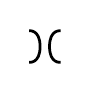
\begin{tikzpicture}[scale=.2]
 \draw [ line width=0.35mm] plot [smooth, tension=2] coordinates { (-1,-1) (-0.3, 0) (-1,1)};
 \draw [ line width=0.35mm] plot [smooth, tension=2] coordinates { (1,-1) (0.3, 0) (1,1)};
 \end{tikzpicture}}\, \rangle \label{regbracket1} \\
&&\langle K \sqcup \bigcirc \rangle = \left (-A^2 - A^{-2}\right ) \langle K \rangle \\
&&  \langle \, \bigcirc \, \rangle  = 1 
\end{eqnarray}

The first axiom gives the smoothing rule on a local region of the knot diagram. This means that  all three diagrams in \ref{regbracket1} are identical everywhere except in the region that is shown inside the brackets. The second axiom tells us that a disjoint circle from the rest of the diagram multiplies the diagram by $(-A^2 - A^{-2})$. The last axiom is the basis of the inductive process. Note that the Kauffman bracket polynomial is invariant under the second and the third Reidemeister moves but not under the first Reidemeister move. In order to establish invariance under the first move,  we choose an orientation for the knot diagram, i.e. we assign a direction indicated by arrows on its arcs. The crossings in an oriented diagram are given signs of $\pm 1$ (see Fig.~\ref{crossings})

\begin{figure}[h]
\centering
\subfloat[]{
 \raisebox{-.1cm}{
\begin{tikzpicture}[scale=.5]
\draw [line width=0.8mm]  (-1,-1)-- (-0.22,-0.22);
\draw  [line width=0.8mm](-1,1)--(0,0);
\draw  [line width=0.8mm] (0.22,0.22) -- (1,1)[->];
\draw [line width=0.8mm]   (0,0) -- +(1,-1)[->];
\end{tikzpicture}}}   \hspace{3cm}
\subfloat[]{ \raisebox{-.1cm}{
\begin{tikzpicture}[scale=.5]
\draw  [line width=0.8mm] (-1,-1)-- (0,0) ;
\draw [line width=0.8mm] (-1,1)--(-0.22,0.22);
\draw [line width=0.8mm] (0,0) -- (1,1)[->];
\draw [line width=0.8mm]   (0.22,-0.22) -- +(.8,-.8)[->];
\end{tikzpicture}}}
\caption{A positive crossing with sign +1 (a) and a negative crossing with sign -1 (b).}\label{crossings}
\end{figure}

The sum of signs of all crossings of a knot diagram $K$ is called {\it the writhe} of $K$, ${\rm wr}(K)$, and it will allow us to make the Kauffman bracket invariant under the first Reidemeister move. Indeed, by considering the following normalization of the Kauffman bracket,  we have achieved our goal.
\begin{equation}\label{jones}
f_K(A) = (-A^3)^{- {\rm wr}(K)} \langle K \rangle,
\end{equation}
where $\langle K \rangle$ is the Kauffman bracket polynomial of $K$. It turns out the $f_K(A)$ coincides with the classical Jones polynomial.

\subsubsection{\label{sec:theory:jones:jonesknotoids}Jones polynomial for knotoids}
One may extend the definition of the Kauffman bracket and, in turn of the classical Jones Polynomial, to the case of knotoids. The rules are more or less the same, with some minor tweaks depending on whether we want compute the invariant for a knotoid in $S^2$ or a planar knotoid. Knotoids are open ended diagrams and therefore when one smoothes all crossings of the diagram, in the end they will always end up with a number of disjoint circles and a single long segment. We choose the long segment to be the basis of the inductive procedure and so the axioms for a knotoid diagram $k$ become as follows:
\begin{eqnarray}
&&\langle \raisebox{-.1cm}{
\begin{tikzpicture}[scale=.2]
\draw [line width=0.35mm]  (-1,-1)-- (-0.22,-0.22);
\draw  [line width=0.35mm ](-1,1)--(0,0);
\draw  [line width=0.35mm] (0.22,0.22) -- (1,1);
\draw [line width=0.35mm]   (0,0) -- +(1,-1);
\end{tikzpicture}}\, \rangle =A \langle \, \raisebox{-.07cm}{
\begin{tikzpicture}[scale=.2]
\draw [line width=0.35mm] plot [smooth, tension=2] coordinates { (-1,.8) (0, 0.5) (1,.8)};
\draw [ line width=0.35mm] plot [smooth, tension=2] coordinates { (-1,-.8) (0, -0.5) (1,-.8)};
\end{tikzpicture}}\, \rangle   + A^{-1} \,\langle\, \raisebox{-.1cm}{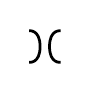
\begin{tikzpicture}[scale=.2]
 \draw [ line width=0.35mm] plot [smooth, tension=2] coordinates { (-1,-1) (-0.3, 0) (-1,1)};
 \draw [ line width=0.35mm] plot [smooth, tension=2] coordinates { (1,-1) (0.3, 0) (1,1)};
 \end{tikzpicture}}\, \rangle  \\
&&\langle k \sqcup \bigcirc \rangle = \left (-A^2 - A^{-2}\right ) \langle k \rangle\\
&&  \langle \, \raisebox{.07cm}{
\begin{tikzpicture}[scale=.1, baseline]
\draw[line width=0.35mm] 
  (1,0) 
    .. controls (3,2) and (5,-2) .. 
  (7,0);  
\draw[black,fill=black] (1,0) circle (2ex);
\draw[black,fill=black] (7,0) circle (2ex);
\end{tikzpicture}}\, \rangle  = 1 \label{regbracket3}
\end{eqnarray}

The invariance unde the first Reidemeister move is taken care by the same normalization as with the case of knots.
\begin{equation}\label{jonesknotoids}
J_k(A) = (-A^3)^{- {\rm wr}(k)} \langle k \rangle,
\end{equation}

where $\langle k \rangle$ is the Kauffman bracket polynomial of a knotoid diagram $k$ and ${\rm wr}(k)$ is the writhe of $k$. Equation~\ref{jonesknotoids} is the extension of the classical Jones for the case of knotoids in $S^2$.
\subsubsection{\label{sec:theory:jones:jonesknotoids}Turaev loop bracket polynomial for planar knotoids}
The case of planar knotoids requires some more explanation. As mentioned above when one smoothes all crossings of a knotoid diagram, they will end up with a number of disjoint circles and one long segment. When we work on the surface of a 2-sphere, it doesn't matter whether the long segment rests inside a circle or not because, even if it does, we can always take it out by moving an arc of the circle around the surface of the sphere. If we work with planar knotoids, we cannot do this and so we want to keep track of this information, i.e. if the long segments is inside a circle or not. For this reason, we add an extra variable to the Kauffman bracket polynomial that counts the number of circles that enclose the long segment in each possible smoothing of the knotoid diagram $k$.

\begin{eqnarray}
&&\langle \raisebox{-.1cm}{
\begin{tikzpicture}[scale=.2]
\draw [line width=0.35mm]  (-1,-1)-- (-0.22,-0.22);
\draw  [line width=0.35mm ](-1,1)--(0,0);
\draw  [line width=0.35mm] (0.22,0.22) -- (1,1);
\draw [line width=0.35mm]   (0,0) -- +(1,-1);
\end{tikzpicture}}\, \rangle_{\circ}=A \langle \, \raisebox{-.07cm}{
\begin{tikzpicture}[scale=.2]
\draw [line width=0.35mm] plot [smooth, tension=2] coordinates { (-1,.8) (0, 0.5) (1,.8)};
\draw [ line width=0.35mm] plot [smooth, tension=2] coordinates { (-1,-.8) (0, -0.5) (1,-.8)};
\end{tikzpicture}}\, \rangle_{\circ}   + A^{-1} \,\langle\, \raisebox{-.1cm}{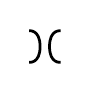
\begin{tikzpicture}[scale=.2]
 \draw [ line width=0.35mm] plot [smooth, tension=2] coordinates { (-1,-1) (-0.3, 0) (-1,1)};
 \draw [ line width=0.35mm] plot [smooth, tension=2] coordinates { (1,-1) (0.3, 0) (1,1)};
 \end{tikzpicture}}\, \rangle_{\circ} \label{regbracket1} \\
&&\langle K \sqcup \bigcirc \rangle_{\circ} = \left (-A^2 - A^{-2}\right ) \langle K \rangle_{\circ} \label{regbracket2}\\
&&\langle \ 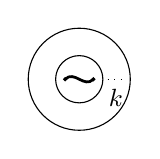
\begin{tikzpicture}[scale=.06,baseline]
        \draw (4,0) circle (5);
        \draw (4,0) circle (10.8);
         \draw[line width=0.35mm] 
  (1,0) 
    .. controls (3,2) and (5,-2) .. 
  (7,0);  
\draw[black,fill=black] (1,0) circle (2ex);
\draw[black,fill=black] (7,0) circle (2ex);
\draw[dotted] (0:10) -- node[below] {{\small $k$}} (0:13.5);
           \end{tikzpicture}
           \
            \rangle_{\circ} = v^k \label{regbracket3}\\
&&  \langle \, \raisebox{.07cm}{
\begin{tikzpicture}[scale=.1, baseline]
\draw[line width=0.35mm] 
  (1,0) 
    .. controls (3,2) and (5,-2) .. 
  (7,0);  
\draw[black,fill=black] (1,0) circle (2ex);
\draw[black,fill=black] (7,0) circle (2ex);
\end{tikzpicture}}\, \rangle_{\circ}  = 1 \label{regbracket4}
\end{eqnarray}

This version of the bracket is a Laurent polynomial in $\mathbb{Z}[A,A^{-1},v]$. The invariance under the first Reidemeister move is given again by the same normalization:
\begin{equation}\label{loopbracket}
\widehat{J}_k(A, v) = (-A^3)^{- {\rm wr}(k)} \langle k \rangle_{\circ},
\end{equation}
where $ \langle k \rangle_{\circ}$ is an evaluation of the diagram $k$ using the rules described above.  The Turaev loop bracket polynomial is  defined by the Equation~\ref{loopbracket} and is an extension of the classical Jones polynomial to the case of planar knotoids.

\subsubsection{The arrow polynomial}

The arrow polynomial is based on the oriented expansion of the bracket polynomial and it was initially  defined in \cite{dye2009} as an invariant for virtual knots. It is a Laurent polynomial in the ring $\mathbb{Z}[A^{\pm1}, L_1, L_2, \ldots ]$, where the $L_i$ are an infinite set of independent commuting variables that also commute with the
Laurent polynomial variable $A$. The extension to classical knotoids in $S^2$ and virtual knotoids appeared in \cite{guka}. The skein relation in this case involves  smoothings with matching or conflicting orientations (see Eqs.~\ref{eq:arrow1} - \ref{eq:arrow5}).
\begin{eqnarray}
&&\raisebox{-0.5\height}{\includegraphics{arrow_skeinrelations_1}} \label{eq:arrow1}\\
&&\raisebox{-0.5\height}{\includegraphics{arrow_skeinrelations_2}}\label{eq:arrow2}\\
&&\raisebox{-0.5\height}{\includegraphics{arrow_skeinrelations_3}}\label{eq:arrow3}\\
&&\raisebox{-0.5\height}{\includegraphics{arrow_skeinrelations_4}}\label{eq:arrow4}\\
&&\raisebox{-0.5\height}{\includegraphics{arrow_skeinrelations_5}}\label{eq:arrow5}
\end{eqnarray}


 Note that each smoothing with a conflicting orientation results in a pair of cusps and, therefore, the set of axioms  for the recursive definition of the arrow polynomial \`{a} la bracket polynomial has to include rules that take into account these additional combinatorial structures. Each state includes a number of circular components and a long segment component, all of which may contain a number of consecutive cusps. A cancellation rule allows the simplification of two consecutive cusps into a straight arc, if the acute angles of both cusps are in the same local region of the diagram (see Fig.~\ref{fig:cancel}). The cancellation rule is not applicable to cases where the acute angles of two consecutive cusps are in different local regions of the diagram. 
 The arrow polynomial assigns a new variable to each long segment of a state with a number of surviving cusps. In particular, two consecutive surviving cusps form a zigzag and a long segment with $2i$ surviving cusps is evaluated at $m_i$. The skein relation together with the axioms discussed above define recursively the arrow polynomial. The arrow polynomial becomes an ambient isotopy invariant under the following normalization:

\begin{equation}\label{eq:arrow}
\mathcal{A}(k) = \left( - A^3 \right )^{-{\rm wr}(k)} \left [ k  \right ],
\end{equation}
where $ \left [ k  \right ]$ is an evaluation of the diagram $k$ using the rules described above.
 \begin{figure}[h] 
\centering
\includegraphics{figure_9}
\caption{\footnotesize The allowed and the forbidden cancellation rules.}\label{fig:cancel}
\end{figure}

\subsubsection{The loop arrow polynomial}

In analogy to the Turaev loop bracket, the loop arrow polynomial is the planar version of the arrow polynomial and it was mentioned first in \cite{gound2}. It is also a Laurent polynomial and it is lies in the ring 
\[
\mathbb{Z}[A^{\pm1}, v, m_1, m_2, \ldots, w_1, w_2, \ldots, p_1, p_2 \ldots, q_1, q_2, \ldots ],
\] where the $m_i$, $w_j$, $p_k$, $q_\ell$ are infinite sets of independent commuting variables that also commute with the
Laurent polynomial variables $A$ and $v$.  The loop arrow distinguishes two different types of zigzags (compare the zigzags in Eq.~\ref{eq:arrow4} to those in Eqs.~\ref{eq:loop_arrow1} and \ref{eq:loop_arrow2}) and it assigns one of the variables  $m_k$ or $w_i$, depending on the type of zigzag. Furthermore, much like the Turaev loop bracket, the loop arrow polynomial assigns different variables to circular components that enclose the long segment with or without any of the two types of zigzags. The loop arrow polynomial is defined by the rules of the arrow polynomial plus the additional rules in in Eqs.~\ref{eq:loop_arrow1}-\ref{eq:loop_arrow5}. 
\begin{eqnarray}
&&\raisebox{-0.5\height}{\includegraphics{loop_arrow_skeinrelations_1}}\label{eq:loop_arrow1}\\
&&\raisebox{-0.5\height}{\includegraphics{loop_arrow_skeinrelations_2}}\label{eq:loop_arrow2}\\
&&\raisebox{-0.5\height}{\includegraphics{loop_arrow_skeinrelations_3}}\label{eq:loop_arrow3}\\
&&\raisebox{-0.5\height}{\includegraphics{loop_arrow_skeinrelations_4}}\label{eq:loop_arrow4}\\
&&\raisebox{-0.5\height}{\includegraphics{loop_arrow_skeinrelations_5}}\label{eq:loop_arrow5}
\end{eqnarray}

Note that the type of zigzag that is evaluated at $m_k$ by the loop arrow polynomial while the arrow polynomial evaluates it at $L_k$. Since this is, in fact, the same rule and since what only changes is the variable that we use, we choose to use the variable $m_k$ when working with the loop arrow polynomial. Finally, as usual, the following normalization turns the loop arrow polynomial into an ambient isotopy invariant:

\begin{equation}\label{eq:arrow}
\widehat{\mathcal{A}}(k) = \left( - A^3 \right )^{-{\rm wr}(k)} \left [ k \right ]_{\circ},
\end{equation}
where $ \left [ k  \right ]_{\circ}$ is an evaluation of the diagram $k$ using the rules described above.



\subsection{\label{sec:theory:notations}Notation Conventions}
Knots have been tabulated in terms of number of crossings\cite{Rolfsen1976,Adams,dowker1983,hoste1998}. The standard notation is in the form $X_Y$ or $X\_ Y$, where $X$ is the number of crossings of the knot diagram in question and $Y$ corresponds to the position of the knot in the table among knots with the same number of crossings. For example, $5_2$ or $5\_2$ denotes the second knot in the knot table that has five crossings. An ``m'' is added at the end of a knot name when its mirror image is considered. The mirror image transforms a knot into a knot represented by the same diagrams with overpasses changed to underpasses and vice versa\cite{Adams}. For example $3_1^m$ or $3\_1m$ is the mirror image of the knot $3_1$. Additionally, we use * to denote the connected sum of two knots, for instance $3_1$*$5_2$ is the product between a $3_1$ and a $5_2$ knot.

The same notation is also implemented for the case of knotoids. There are three symmetry related operations that can be applied on a knotoid diagram. First is the mirror reflection, the equivalent of the mirror image of a knot, that changes overpasses to underpasses and vice versa \cite{turaev}. The mirror image of a knotoid $K$ is denoted by $Km$ (Figure~\ref{fig:involutions} bottom-left). The second operation is the symmetric involution which corresponds to the two dimensional reflection. The symmetric of a knotoid $K$ is denoted by $Ks$ (Figure~\ref{fig:involutions} top-right). Finally, the mirror symmetric of a knotoid is the composition of the above two involutions and can be seen as a rotation by an angle $\pi$ around the axis that passes through the endpoints of the knotoid and it is denoted by $Kms$ (Figure~\ref{fig:involutions} bottom-right). For the product of two knotoids we use *, the same symbol with the connected sum of two knots. For instance, $2_1$*$3_1$ is the product between a $2_1$ and a $3_1$ knotoid.
\begin{figure}[h]
\centering
\includegraphics{involutions}
\caption{Knotoid $2_1$ with its symmetric $2_1s$, mirror $2_1m$ and mirror symmetric $2_1ms$.}\label{fig:involutions}
\end{figure}


A table with knotoids on the sphere with up to 5 crossings already exists\cite{bartholomew}. However, here\footnote{when using internal database with \lstinline{--names-db=internal} or with files \lstinline{examples/knotoid_names_planar.txt}, \lstinline{examples/knotoid_names_sphere.txt}, \lstinline{examples/knotoid_names_planar_arrow.txt} or \lstinline{examples/knotoid_names_sphere_arrow.txt}} we use a different table based on a complete classification of all knotoids on the plane with up to 5 crossings and of all knotoids on the sphere with up to 6 crossings (see \cite{goundaroulis2019} for more details).

\subsection{\label{sec:theory:knottedcore}Knotted proteins, slipknots and knotted cores}

It is a long standing belief that folded configurations of proteins should provide an insight on the folding pathways that the backbone follows to reach its native state\cite{Crippen74, Connolly80}. In principle, proteins tend to avoid folding into configurations that involve non-trivial topological features such as knots. At a first glance, it may appear as if nature selects with a bias against the formation of knots. However, their existence\cite{taylor2000} tells us that this may not be the case as knots have been observed to contribute in the stability as well as the function of a protein.

A fingerprint matrix is a triangular matrix where  each entry $(i,j)$ corresponds to a subchain with starting index $i$ and ending index $j$, while it carries also the information of the dominant knotoid or knot type  of its corresponding subchain and it is encoded using a colour scale. Moreover, the whole chain corresponds to the lower left part of the matrix and, therefore, the fingerpring matrix provides a detailed overview of the global as well as the local topology of an open chain.
The knotted core is defined as the shortest subchain obtained by progressively altering the length of the whole chain by 1 point without changing the knot(oid) type in the process. Visually, the knotted core is the  point of the path connected region that includes  the full chain and is closer to the diagonal of the fingerprint matrix. In Figure~\ref{fig:3KZN:fingerprint1000} we see the knotoid fingerprint for the protein 3KZN. Note that this definition of the knotted core corresponds to the "top-down" knotted core discussed by Tubiana and coauthors \cite{tubiana2011}.



In open chains the ending index has to be greater than the starting index which leads to the empty upper part of the matrix and thus to the triangular shape of the fingerprint. On the other hand, in closed chains there is not such a restriction\cite{rawdon,rawdon2}. Thus disk matrices provide an ideal representation of the topology closed chains. In this case we use polar coordinates $(r, \theta)$ to read the matrices, where $r$ corresponds to the length of the subchain and $\theta$ corresponds to the midpoint of the subchain (see Figure~\ref{fig:3KZN:disk}). In analogy to the fingerprint matrix, the knotted core is the  point of the path connected region that includes  the full chain and is closer to the center of the disk matrix.

Apart from knotoids and knots, slipknots also seem to provide valuable information on protein folding\cite{yeates}. Slipknotting appears when a part of the protein backbone forms a knot and then it doubles back so that a non-minimal diagram of the unknot is formed\cite{yeates}. Slipknots can be also generalized to the case of knotoids, where the only difference lies in the fact that the chain may also correspond to a non-minimal non-trivial knotoid. In order to detect slipknots, one has to study all possible subchains of the initial chain. Each subchain is evaluated for the knot or the knotoid type it posseses and the results are summarized in the fingerprint\cite{yeates, sulkowska2012,gound} or disk matrix\cite{rawdon}.
A slipknot can then be visualized as a  region of the matrix that corresponds to a non-trivial knot(oid) and  is disconnected from the region containing the full chain.



\clearpage



\bibliographystyle{unsrt} 
\bibliography{bibliography}

\end{document}

